% -*- root: ../EDP2016.tex -*-
% clase 2016/02/15

\chapter{Ecuaciones de segundo orden. Series de Fourier}
\label{chap:EcuacionesSegundoOrden}

\section{Método de separación de variables}\index{Ecuación! del calor}

	Al empezar el curso ya vimos un ejemplo: la ecuación del calor en una dimensión con datos de contorno Dirichlet homogéneos.\index{Método!separación de variables}

	\begin{example} \concept{Ecuación \IS con contorno Dirichlet}
		\[
		\begin{cases}
		u_t - u_{xx} = 0 & x \in (0,L), \quad t > 0 \\
		u(0,t) = u(L,t) = 0 & t > 0 \\
		u(x,0) = f(0) & x \in [0,L]
		\end{cases}
		\]

		La ecuación del medio es el dato de contorno de Dirichlet\index{Condición! de contorno Dirichlet} homogéneo, es decir, que especifica el dato en los extremos.

		Llegamos con separación de variables a que la solución del problema podía ser escrita como:

		\[ u(x,t) \eqexpl{?} \sum^{\infty}_{k=1} a_k e^{-(\frac{k\pi}{L})^2 t} \sin \left( \frac{k\pi}{L} x \right) \]
		donde
		\[ f(x) \eqexpl{?} \sum^{\infty}_{k=1} a_k \sin \left( \frac{k\pi}{L}x \right) \]
	\end{example}


	\begin{example} \concept{Ecuación \IS con contorno Neumann}

		\[
		\begin{cases}
		u_t - u_{xx} = 0 & x \in (0,L), t > 0 \\
		u_x(0,t) = u_x(L,t) = 0 & t > 0 \\
		u(x,0) = f(x) & x ∈ \in [0,L]
		\end{cases}
		\]

		Esta condición indica que no hay flujo de calor entre la varilla y cualquier punto fuera, incluidos los extremos. Esperamos que al final, cuando el tiempo tienda a infinito el calor se haya distribuido a lo largo de la varilla y la temperatura sea constante a lo largo de esta. El valor de esto probablemente sea el promedio.

		\begin{figure}[thbp]
		\centering
		\inputtikz{transmisionCalorNeumann}
		\caption{}
		\label{fig:transmisionCalorNeumann}
		\end{figure}

		Empecemos con el método de separación de variables. Buscamos $u(x,t) = X(t) \cdot T(t)$ que sea solución de la ecuación con el contorno (el dato inicial se tratará después).


		\[
		\begin{array}{l}
			0 = u_t - u_{xx} = T' X - T X'' \\
			0 = u_x (0,t) = T(t) X'(0) \\
			0 = u_x (L,t) = T(t) X'(L)
		\end{array}
		\]

		De lo que obtenemos:

		\[ \frac{T'(t)}{T(t)} = \frac{X''(x)}{X(x)} \quad \forall x, \forall t \]

		Como estamos igualando dos cocientes de funciones de variables diferentes que es cierto $\forall x, \forall t$, esto solo puede significar que ambos cocientes son constantes. A esta proporción la llamaremos $\lambda$:

		\[ \frac{T'}{T} = \frac{X''}{X} = \lambda \in \mathbb{R} \]

		% Método general? SI
		Resolvemos la EDO en X:

		\[
		\left\{ \begin{array}{l}
		X'' = \lambda X \\
		X'(0) = X'(L) = 0
		\end{array} \right. \quad\quad \text{(problema de contorno)}
		\]

		Veamos carios casos en función de $\lambda$:

		\begin{itemize}
			\item $\lambda = 0$

				Cuando $\lambda = 0 \Rightarrow X'' = 0$. Así que tenemos que $X'$ tiene que ser constante y $X$ lineal. Pero además los datos iniciales nos indican el valor de $X'$, al ser constante.

				\[ \left.
				\begin{array}{l}
					X(x) = a + bx \\
					\left.
					\begin{array}{r}
						X'(x) = b \\
						X'(0) = X'(L) = 0
					\end{array} \right\} \Rightarrow b = 0
				\end{array} \right\} \Rightarrow X \equiv a \]

				Tiene una solución no trivial que es $\lambda = 0, X=a_0$.

			\item $\lambda > 0$ con $\lambda = \mu^2$, $\mu \in \mathbb{R}$

				Lo cual nos lleva a una EDO de orden 2, que se resolvería con el polinomio característico.

				\[ \text{Las soluciones siguen } \left\{
				   \begin{array}{l}
				   	X(x) = a \cdot e^{\mu x} + b \cdot e^{-\mu x} \\
				   	X'(x) = \mu (a\cdot e^{\mu x} - b\cdot e^{-\mu x})
				   \end{array} \right.
				\]

				\[ \left. \begin{array}{l}
					0 = X'(0) \Rightarrow \mu(a - b) = 0 \\
					0 = X'(L) \Rightarrow \mu(a \cdot e^{\mu L} - b \cdot e^{-\mu L}) = 0
				\end{array} \right\}
					\Rightarrow … \Rightarrow a = b = 0
				\]


			\item $\lambda < 0$ con $\lambda = - \mu^2$

				Aquí volvemos a emplear el polinomio característico pero llegaremos a soluciones complejas.

			 	\[ \text{Solución} \left\{
				   \begin{array}{l}
				   	X(x) = a \cos(\mu x ) + b \sin( \mu x) \\
				   	X'(x) = -a \mu \sin(\mu x) + b \mu \cos(\mu x)
				   \end{array} \right.
				\]

			 	\[
			 		\begin{array}{l}
			 		0 = X'(0) = b \mu \\
			 		0 = X'(L)
			 		\end{array} \Rightarrow b = 0 \Rightarrow \left\{ \begin{array}{l}
			 			X(x) = + a \cos (\mu x ) \\
			 			X'(x) = -a \mu \sin (\mu x)
			 		\end{array} \right.
			 	\]

			 	De lo que obtenemos que

			 	\[0 = X'(L) = -a \mu \sin(\mu L) \Rightarrow \mu L = k \pi , \quad k = 1,2,…\]



		\end{itemize}

		Conclusión:
				\begin{align*}
					\lambda_0 = 0\quad & \quad X_0 = a_0 \\
					\lambda_k = - \left(\frac{k\pi}{L}\right)^2\quad & \quad X_k(x) = a_k \cos \left(\frac{k \pi}{L}x\right)
				\end{align*}

			 	EDO para T (para las $\lambda$ encontradas antes)

			 	\[\lambda_0 = 0 \Rightarrow T'_0 \equiv 0 \Rightarrow T_0 \equiv \alpha_0\]
			 	\[\lambda_k = - \left(\frac{k\pi}{L}\right)^2 \Rightarrow T'_k = -\left(\frac{k\pi}{L}\right)^2 T_k \Rightarrow T_k (t) = \alpha_k e^{-\left(\frac{k\pi}{L}\right)^2 t} \]

			 	Soluciones particulares:
			 	\[u_0(x,t) = A_0, \quad u_k (x,t) = A_k e^{-\left(\frac{k \pi}{L} \right)^2 t} \cos \left( \left( \frac{k \pi}{L}\right) x \right) \]

			 	Dato inicial: $u(x,0) = f(x)$

			 	Idea: $u(x,t) \eqexpl{?} A_0 + \sum\limits_{k=1}^{\infty} A_k e^{- \left( \frac{k \pi}{L} \right)^2 t}  \cos \left( \frac{k \pi}{L} x \right)$

			 	Pero claro, no sabemos calcular $A_k$. ¿O cómo calculamos la convergencia? ¿Cómo calculamos las derivadas?


		\end{example}

		\begin{example}{3: Cuerda vibrante}

			Veamos una cuerda de guitarra en tensión. La guitarra está atada en los extremos y la altura sobre el eje horizontal es $u$.

			\begin{figure}[thbp]
			\centering
			\inputtikz{cuerdaGuitarra}
			\caption{}
			\label{fig:cuerdaGuitarra}
			\end{figure}


			\[  \begin{cases}
				u_{tt} - u_{xx} = 0 \quad \text{ 2º orden \quad 2 datos } \\
				u(0,t) = u(L,t) = 0 \quad \text{Dirichlet}\\
				u(x,0) = f(x) \\
				u_t(x,0) = g(x)
				\end{cases}
			\]

			Por separación de variables. Buscamos un $u(x,t) = X(t) T(t)$, solución de la ecuación con el contorno:
			\[ 0 = u_{tt} - u_{xx} = T'' X - T X''\]
			\[ \frac{T''}{T} = \frac{X''}{X} = \lambda \in \mathbb{R}\]

			EDO para $X$:

			\[\begin{cases}
				X'' = \lambda X \\
				X(0) = X(L) = 0
			\end{cases}
			\]

			Vemos que ha cambiado respecto al sistema anterior en que la última ecuación ya no relaciona las derivadas de $X$ sino $X$. De nuevo, buscamos las soluciones en función del valor de $\lambda$:

			\begin{itemize}
				\item $\lambda = 0$

					\[
					\left\{
					\begin{array}{l}
					X(x) = a + bx \\
					X(0) = 0 = X(L)
					\end{array}
					\right.
					\Rightarrow
					a = 0 = b
					\]

				\item $\lambda > 0$ con $\lambda = \mu^2$

					\[
					\left\{
					\begin{array}{l}
					X(x) = a \cdot e^{\mu x} + b \cdot e^{-\mu x} \\
					X(0) = 0 = X(L)
					\end{array}
					\right.
					\Rightarrow … \Rightarrow
					a = b = 0
					\]

				\item $\lambda < 0$ con $\lambda = -\mu^2$

					\[
					\left\{
					\begin{array}{l}
					X(x) = a\cos(\mu x) + b\sin(\mu x) \\
					X(0) = 0 = X(L)
					\end{array}
					\right.
					\Rightarrow X(0) = a \Rightarrow X(x) = b \sin(\mu x)
					\]

					\[ \Rightarrow X(L) = 0 = b \sin (\mu L) \Rightarrow \mu = \frac{k \pi}{L}\]

			\end{itemize}

			Con lo que llegamos a las soluciones no triviales:

			\[\lambda_k = - (\frac{k\pi}{L})^2, \quad X_k(x) = b_k \sin \left(\frac{k\pi}{L} \right) x\]


			Una vez que resolvemos la EDO para $X$, la resolvemos para $T$:

			\[T'' = \lambda T\]

			Es similar a la X así que tenemos:

			\[T''_k = - (\frac{k\pi}{L})^2 T_k \Rightarrow T_k (t) = \alpha_k \cos\left( \frac{k \pi}{L} t \right) + \beta_k \sin \left( \frac{k \pi}{L}t \right)\]

			Con lo que llegamos a las soluciones particulares:

			\[u_k(x,t) = A_k \cos \left(\frac{k\pi}{L} t\right) \sin \left(\frac{k\pi}{L}x\right) + B_k \sin \left(\frac{k\pi}{L}t\right)  \sin \left(\frac{k\pi}{L}x\right) \]

			Idea: Buscar

			\[u(x,t) \eqexpl{?} \sum_{k=1}^{\infty} A_k \cos \left(\frac{k\pi}{L} t\right) \sin \left(\frac{k\pi}{L} x  \right)+ B_k \sin \left(\frac{k\pi}{L}t \right) \sin \left(\frac{k\pi}{L}  x \right)\]

			Datos iniciales:
			\[ f(x) = u(x,0) \eqexpl{?} \sum^{\infty}_{k=1} A_k \sin \left(\frac{k\pi}{L} x  \right)\]

			Suponiendo que derivada e integral conmutan:

			\[ u_t (x,t) \eqexpl{?} \sum_{k} - A_k \left(\frac{k\pi}{L} \right) \sin \left(\frac{k\pi}{L}t \right) \sin \left(\frac{k\pi}{L}x \right) + B_k \left(\frac{k\pi}{L} \right) \cos \left(\frac{k\pi}{L}t \right) \sin \left(\frac{k\pi}{L}x \right)
			\]

			\[g(x) = u_t(x,0) \eqexpl{?} \sum_k B_k  \left(\frac{k\pi}{L} \right) \sin \left(\frac{k\pi}{L}x \right)\]

		\end{example}

		% clase 2016/02/16

		\begin{example}{4: Ondas con condiciones periódicas}\index{Ecuación!de ondas}\label{ec:ondas}

			Estudiemos, por ejemplo, las olas en alta mar. No tenemos un contorno fijo como antes, así que vamos a buscar soluciones que sean periódicas en los extremos. En este caso tendremos dos condiciones, llamadas condiciones de periodicidad\index{Condición! de periodicidad}. Hemos puesto dos porque lo observamos en segundo orden:

			\[u(-L,t) = u(L,t), \forall t\]
			\[u_x(-L,t) = u_x(L,t), \forall t\]

			El problema nos queda así:

			\[  \begin{cases}
				u_{tt} - u_{xx} = 0 \quad x  \in (-L,L)\footnotemark, t>0\\
				u(-L,t) = u(L,t), \forall t\\
				u_x(-L,t) = u_x(L,t), \forall t
				u(x,0) = f(x) \\
				u_t(x,0) = g(x)
				\end{cases}
			\]
			\footnotetext{Para que las cuentas cuadren mejor}

			Aplicamos el método de separación de variables:
			\[ \frac{T''}{T} = \frac{X''}{X} = \lambda \in \mathbb{R}\]

			EDO para $X$:
			\[\left\{\begin{array}{l}
				X'' = \lambda X \quad x \in (-L,L) \\
				X(-L) = X(L) \\
				X'(-L) = X'(L)
			\end{array}
			\right. \]

			\begin{itemize}
				\item $\lambda = 0$
					\[\left\{\begin{array}{l}
						X = a+bx \\
						X'(x) = b \\
						X(-L) = X(L) \quad \Rightarrow a + b(-L) = a + bL \Leftrightarrow b = 0
					\end{array}
					\right. \]

					Si $b = 0$ entonces la $a$ será arbitraria. $\Rightarrow \lambda_0 = 0$, $ X_0 \equiv a \in \mathbb{R}$


				\item $\lambda > 0$ con $\lambda = \mu^2$

					\[\begin{cases}
						X(x) = a\cdot e^{\mu x} + b \cdot e^{-\mu x} \\
						X'(x) = a\mu \cdot e^{\mu x} - b \mu \cdot e^{-\mu x}
					\end{cases}
					\Rightarrow a = b = 0 \]


				\item $\lambda < 0$ con $\lambda = -\mu^2$

					\[ X (x) = a \cos (\mu x) + b \sin (\mu x) \]

					\[\text{2 caminos: }\left\{\begin{array}{l}
						\text{ pensar }\rightarrow \mu = \frac{2\pi}{L} \\
						\text{ hacer cuentas }\footnotemark\rightarrow \left\{ \begin{array}{l}
							X(-L) = X(L) \\
							X'(-L) = X'(L)
						\end{array} \right.
					\end{array}
					\right. \]\footnotetext{se dejan como ejercicio}
			\end{itemize}

			Ajustamos $\mu$ para que $X$ sea periódica con periodo $2L k \Rightarrow … \Rightarrow \mu = \frac{k \pi}{L}$. Donde $2L$ es la longitud del intervalo. Por lo que llegamos a las soluciones:

			\[
			\lambda_k = -\left(\frac{k\pi}{L}\right)^2\quad\quad X_k(x) = a_k \cos \left( \frac{k\pi}{L} x \right) + b_k \sin \left( \frac{k\pi}{L} x \right)
			\]

			EDO para $T$:

			\[ \lambda_0 = 0 \rightarrow T''=0 \rightarrow T(t) = \alpha_0 + \beta_0 t\]

			\[ \lambda_k = - \left( \frac{k\pi}{L} \right)^2, \quad T''_k = - \left( \frac{k\pi}{L} \right)^2 T_k \]

			\[\Rightarrow T_k(t) = \alpha_k \cos \left( \frac{k\pi}{L} t \right) + \beta_k \sin \left( \frac{k\pi}{L} t \right) \]

			Soluciones particulares de la EDO para T:

			\[u_k (x,t) = T_k(t) \cdot X_k(x) \quad k = 0,1,2,… \]


			Soluciones en forma de serie:

			\[u(x,t) = \sum_{k=1}^{\infty} u_k (x,t) \rightarrow \text{ Ajustar datos } f,g \]

			¿Converge esta serie?. La ecuación del calor era buena, ya que al tener una exponencial menor que 0 tendía a 0 muy rápido. En la ecuación de ondas la parte temporal no ayuda ya que tiene un comportamiento cualitativo distinto.

			Volvemos a nuestras soluciones particulares:

			\[u_0(x,t) = a_0 + b_0t\]

			% lo siento mucho si hay una errata en estas fórmula y te toca editarlas.

			\begin{align*}
			u_k(x,t) = &\left(\alpha_k \cos \left( \frac{k \pi}{L} t \right) + \beta_k \sin \left( \frac{k \pi}{L} t \right) \right) \\
			\cdot &\left(a_k \cos \left( \frac{k \pi}{L} x \right) + b_k \sin \left( \frac{k \pi}{L} x \right) \right)
			\end{align*}
			\begin{align*}
			u_k(x,t) = &\left(A_k \cos \left( \frac{k \pi}{L} x \right) + B_k \sin \left( \frac{k \pi}{L} x \right) \right) \cos \left( \frac{k \pi}{L} t \right)\\
			+ &\left(C_k \cos \left( \frac{k \pi}{L} x \right) + D_k \sin \left( \frac{k \pi}{L} x \right) \right) \sin \left( \frac{k \pi}{L} t \right)
			\end{align*}




			\[u_k(x,t) = T_k(t) X_k(t) \quad (k=0,1,2,…)\]


			y soluciones en forma de serie:

			\[ u(x,t) = u_0 + \sum_k u_k \]

			\begin{align*}
				u(x,t) = A_0 + C_0 t &+ \sum^{\infty}_{k=1} \left(A_k \cos \left( \frac{k \pi}{L} x \right) + B_k \sin \left( \frac{k \pi}{L} x \right) \right) \cos \left( \frac{k \pi}{L} t \right)\\
				&+ \sum^{\infty}_{k=1} \left(C_k \cos \left( \frac{k \pi}{L} x \right) + D_k \sin \left( \frac{k \pi}{L} x \right) \right) \sin \left( \frac{k \pi}{L} t \right)
			\end{align*}

			En $t = 0$

			\[f(x) = u(x,0) = A_0 + \sum_{k=1}^{\infty} A_k \cos \left( \frac{k \pi}{L} x \right) + B_k \sin \left( \frac{k \pi}{L} x \right) \]

			\[g(x) = u_t (x,0) = C_0 + \sum_{k=1}^{\infty} \left(\frac{k \pi}{L}\right) \left( C_k \cos \left( \frac{k \pi}{L} x \right) + D_k \sin \left( \frac{k \pi}{L} x \right)\right) \]


		\end{example}

		De 4 ejemplos hemos obtenido la misma solución:

		\[ f(x) = \sum_{k=1}^{\infty} b_k \sin \left( \frac{k \pi}{L} x \right), \quad x \in (0,L) \]

		\[ f(x) = a_0 + \sum^{\infty}_{k=1} a_k \cos \left( \frac{k \pi}{L} x \right), \quad x \in (0,L) \]

		\(
		f(x) \qeq a_0 + \sum^{\infty}_{k=1} a_k \cos \left( \frac{k \pi}{L} x \right) + b_k \sin \left( \frac{k \pi}{L} x \right), \quad x \in (-L,L)
		\)

		Ésta última es combinación de las dos anteriores, y nos lleva al problema que queremos resolver. ¿Es una solución?, y en ese caso: ¿Es única?.\\

		\textbf{Recordemos} las ecuaciones del coseno y seno suma:
		\[
		\left. \begin{array}{r}
			\cos (a + b) = \cos a \cos b - \sin a \sin b \\
			\cos (a - b) = \cos a \cos b + \sin a \sin b \\
		\end{array} \right\} \Rightarrow \left\{ \begin{array}{l}
			\cos a \cos b = \frac{1}{2} (\cos (a+b) + \cos (a-b)) \\
			\sin a \sin b = \frac{1}{2} (\cos (a-b) - \cos (a+b))
		\end{array} \right.
		\]

		\[
		\left. \begin{array}{r}
			\sin (a + b) = \sin a \cos b + \cos a \sin b \\
			\sin (a - b) = \sin a \cos b - \cos a \sin b \\
		\end{array} \right\} \Rightarrow \left\{ \begin{array}{l}
			\sin a \cos b = \frac{1}{2} \{\sin (a+b) + \sin(a-b)\}
		\end{array} \right.
		\]

		\begin{figure}[thbp]
		\centering
		\inputtikz{interpretacionDalembert}
		\caption{Interpretación de la ecuación D'Alembert}
		\label{fig:interpretacionDalembert}
		\end{figure}

		Con esto simplificamos (asumiendo ciertas regularidades de las integrales) las expresiones que obteníamos anteriormente y llegamos a la \concept{Fórmula de D'Alembert}:

		\(
		u(x,t) = \frac{1}{2} \left\{ f(x+t) + f(x-t) \right\} + \frac{1}{2} \int^{x+t}_{x-t} g(s) \dif s  \label{eq:DALEMBERT}\)

		Su interpretación puede verse en la figura \ref{fig:interpretacionDalembert}

		Supongamos $g=0$ y $u(x,t) = \frac{1}{2} \{ f(x+t) - f(x-t)\} $


	\section{Nociones sobre convergencia}

	El problema que se abre ante nosotros es calcular el límite de la siguiente suma
	\[ \sum^{\infty}_{k=1} \Phi_k(x) \qeq f(x) \]

 	Por simplificar, generalizaremos un poco: dada una sucesión $f_n$ de funciones\footnote{Para nosotros, lo que tendremos es $f_n = \sum_{k=1}^n Φ_k(x)$, pero así es más sencillo de trabajar.}, ¿qué podemos decir del siguiente límite?
	\[ \lim_{n \rightarrow \infty} f_n(x) \eqexpl{?} f(x) \]

	Para tratar este tema con propiedad, vamos a ver primero algunas nociones sobre convergencia de funciones.

	\subsection{Convergencia puntual}

		La idea más sencilla de convergencia es la puntual: queremos ver que las funciones se acercan una a la otra punto a punto.

		Más formalmente, asumiendo que la sucesión de funciones $f_n$ están definidas en $(a,b)$, fijamos un $x_0 \in (a,b)$ y consideramos la sucesión de números $\set{f_n(x_0)}_{n ∈ ℤ} ⊂ ℝ$. Querremos ver entonces que
		\[ \liminft{n} f_n(x_0) = f(x_0) \quad \forall x_0 \in (a,b)\]

		Esto nos lleva a nuestra primera noción de convergencia.

		\begin{defn}[Convergencia\IS puntual] Dada $\set{f_n}_{n ∈ ℤ}$ una sucesión de funciones, se dice que $f_n$ converge puntualmente a $f$ ($f_n \rightarrow f $ puntualmente) en $(a,b)$ si y sólo si para todo $x \in (a,b)$, dado $\epsilon > 0$ podemos encontrar $n_0$, tal que si $n \geq n_0$, entonces $|f_n(x) - f(x)| < \epsilon$.

			\begin{obs}
				$n_0$ es una función de $\epsilon$ y $x$: $n_0 = n_0(\epsilon, x)$
			\end{obs}

		\end{defn}

		Recordemos que la convergencia puntual no se comporta ``bien'' ni con la continuidad ni con las integrales.

		\begin{example}[De continuidad]
		Nuestra sucesión de funciones continuas será la siguiente:
			\[
			f_n(x) = \begin{cases}
			1 - nx & x \in [0, \frac{1}{n}]\\
			0 & x \in [\frac{1}{n},1]
			\end{cases} \quad \text{ continuo }\forall n
			\], que se puede ver que converge a lo siguiente: \[
			\lim_{n \rightarrow \infty} f_n(x) = \begin{cases}
			1 & x = 0\\
			0 & x \neq 0
			\end{cases}
			\], que es obviamente no continuo.

			\begin{figure}[thbp]
			\centering
			\begin{tikzpicture}[scale = 2]
				\draw[->] (-0.2,0) -- (1.5,0);
				\draw[->] (0,-0.2) -- (0,1.3);

				\draw[red, thick] (0,1) node [black, left] {1} -- (0.5,0) node [black, below] {$\frac{1}{n}$} -- (1,0) node [black, below] {$1$};

				\begin{scope}[xshift = 2.5cm]
				\draw[->] (-0.2,0) -- (1.5,0);
				\draw[->] (0,-0.2) -- (0,1.3);

				\draw[red, thick] (0,1) node [black, left] {1} .. controls (0.1,1.2) and (0.3,0.05) .. (0.7,0) node [black, below] {$\frac{1}{n}$} -- (1,0) node [black, below] {$1$};
				\end{scope}
			\end{tikzpicture}
			\caption{Una muestra de que la sucesión de funciones continuas (incluso $C^∞$, como en el caso de la derecha) da como límite una función no continua.}
			\label{fig:ejemploContinuidadPuntual}
			\end{figure}
		\end{example}

		\begin{example}[De integral]

			\begin{wrapfigure}{R}{0.4\textwidth}
			\centering
			\begin{tikzpicture}[scale = 2]
				\draw[->] (-0.2,0) -- (1.5,0);
				\draw[->] (0,-0.2) -- (0,1.3) node [left] {$f(x)$};

				\draw[red, thick] (0,0) -- (0.5,1) node (T) {} -- (1,0) node [black, below] {$\frac{1}{n}$};

				\draw[dashed] (0, 1) -- (0.5, 1);
				\node[hnlin, label={left:$n$}] at (0,1) {};
			\end{tikzpicture}
			\caption{La función tiene área constante, aunque converge puntualmente a $0$.}
			\label{fig:ejemploContinuidadPuntual2}
			\end{wrapfigure}

			Tomando una función como en la \fref{fig:ejemploContinuidadPuntual2}, vemos que converge puntualmente a $0$ para cualquier $x$, pero \[ \int_0^1 f_n(x) \dif x = \frac{1}{2} \quad \forall n \] y nos queda lo siguiente: \[ \lim_{n \to \infty} \int_0^1 f_n(x) \dif x = \frac{1}{2} \neq \int_0^1 \lim_{n \to \infty} f_n(x)  \dif x = 0  \]

		\end{example}

	\subsection{Convergencia uniforme}

		\begin{figure}[thbp]
		\centering
		\inputtikz{ConvergenciaUniforme}
		\caption{Interpretación geométrica de la convergencia uniforme}
		\label{fig:convergenciaUniforme}
		\end{figure}

		La sección anterior nos da una justificación clara de que necesitamos algo más que sólo convergencia puntual: tenemos que controlar de alguna forma todos los puntos a la vez para evitar problemas con la integral y con la continuidad. Este control será el de la convergencia uniforme.

		\begin{defn}[Convergencia\IS uniforme] $\{f_n\}$ converge a $f$ uniformemente en $(a,b) \Leftrightarrow$ para todo $\epsilon > 0$, podemos encontrar ${n_0 = n_0(\epsilon)}$ tal que si $n \geq n_0$ entonces $|f_n(x) - f(x)| < \epsilon$, $\forall x \in (a,b)$.

		Esta definición es equivalente a decir que
		\[
			\sup_{x \in (a,b)} |f_n(x) - f(x)| < \epsilon
		\iff
			\left.||f_n - f||_{\infty}\right|_{(a,b)} < \epsilon
		\]
		\end{defn}

		Esta definición tiene una \textbf{interpretación geométrica} fácil de ver (\fref{fig:convergenciaUniforme}). Tenemos una banda de tamaño $2\epsilon$ alrededor de toda la gráfica de $f$, y si $n \geq n_0$, {\bf toda} la gráfica de $f_n$ está dentro de dicha banda.

		Como era de esperar, la convergencia uniforme funciona bien con la continuidad y las integrales.

		\begin{theorem}

			Supongamos que $f_n \rightarrow f$ uniformemente en $(a,b)$.

			\begin{itemize}
				\item $f_n$ continuas en $(a,b) \Rightarrow f$ continua en $(a,b)$

				\item $f_n$ integrables, $(a,b)$ acotado

				\[\int^{b}_{a} f(x) dx = \lim_{n \rightarrow \infty} \int^{b}_{a} f_n(x) dx \]
			\end{itemize}

			\obs La convergencia uniforme no preserva la derivabilidad

		\end{theorem}

		\begin{example}{Valor absoluto}

			$\{f_n\}$ funciones ``redondeadas'' que convergen a el valor absoluto. Ver figura \ref{fig:convergenciaValorAbsoluto}

			\begin{figure}[thbp]
			\centering
			\inputtikz{convergenciaValorAbsoluto}
			\caption{Ejemplo de la convergencia uniforme al valor absoluto con funciones derivables.}
			\label{fig:convergenciaValorAbsoluto}
			\end{figure}

			\[f_n(x) = \sqrt{x^2 + 1/n} \convs[][n][\infty] \sqrt{x^2} = |x| \]

		\end{example}

	\subsection{Convergencia en $L^2$}

		Aunque la convergencia uniforme parece que funciona bastante bien, es una continuidad muy fuerte y a veces no necesaria. Una convergencia ``intermedia'' entre la puntual y la uniforme será comprobar simplemente que la integral no se nos descogorcia por completo. Antes de entrar en detalle vamos a dar algunas definiciones.

		\begin{defn}[Espacio\IS de funciones $L^2$] El espacio $L^2((a,b))$ se define como el espacio de funciones integrables\footnote{Mejor dicho, medibles, pero no nos vamos a meter en ese percal en este curso. Para una introducción interesante a estos espacios, ver \citep{ApuntesVarReal}.} cuyo cuadrado tiene integral finita. Es decir, \[ L^2((a,b)) = \set{ \appl{f}{(a,b)}{ℝ} \tq \int_a^b \abs{f(x)}^2 \dif x < ∞ }\]
		\end{defn}

		Este espacio es un espacio vectorial, en el que hay una norma \[ \norm{f}_2 = \left( \int^{b}_{a} |f|^2 \dif x \right)^{\frac{1}{2}}\], un producto escalar asociado (compatible con la norma) \[ \pesc{f,g} = \int^b_a f(x) g(x) \dif x  \] y, por supuesto, una noción de convergencia que es la que tenemos en cualquier espacio normado.

		\begin{defn}[Convergencia\IS en $L^2$] Dadas $\set{f_n}_{n ∈ ℤ} ⊂ L^2$ y $f ∈ L^2$, se dice $f_n$ converge a $f$ en $L^2$ ($f_n \convs[L^2][n] f$) si y sólo si \[ \lim_{n\to ∞} \norm{f_n - f}_2 = 0\]
		\end{defn}

		Un resultado interesante en $L^2$ es que las funciones continuas son densas en él. Es decir, que si cogemos las funciones $C((a,b))$ y añadimos todos los límites de sucesiones de Cauchy, nos queda $L^2$. Esto nos será útil para el futuro, ya que nos permitirá decir que cualquier función $f ∈ L^2$ se puede aproximar como una sucesión de funciones $f_n$ continuas.

		Aunque no lo necesitaremos mucho, podemos definir la norma $L^p$ y su convergencia correspondiente.

		\begin{defn}[Convergencia\IS en $L^p$]
			\[L^p \rightarrow \|f\|_{p} = \left( \int^{b}_a |f|^p \dif x \right)^{\frac{1}{p}} \text{ para } 1 \leq p < \infty \]
		\end{defn}

		\begin{defn}[Convergencia\IS en $L^∞$] La norma infinito es el supremo, de tal forma que la convergencia en este caso es \[ f_n \convs[L^∞][n] f \iff \lim_{n\to ∞} \norm{f_n - f}_∞ = \lim_{n\to ∞} \sup_{x ∈ (a,b)} \abs{f_n(x) - f(x)} = 0\]
		\end{defn}

		\obs Si $p\neq 2$, en $L^p$ no hay producto escalar, y las cuentas se complican.
			Podría ser interesante estudiar para qué valores de $p$ las series de Fourier convergen, pero esto se sale del alcance de esta asignatura.

	% clase 2016/02/17

	\subsection{Relaciones entre las convergencias}

		Una vez que sabemos qué tipos de convergencias vamos a trabajar, nos interesará saber obviamente la relación entre ellas.

		Por ejemplo, es trivial ver que la convergencia uniforme implica convergencia puntual.

		\begin{wrapfigure}[12]{R}[0.15\textwidth]{0.4\textwidth}
		\vspace{-10pt}
		\inputtikz{ConvergenciaUniformeNoL2}
		\vspace{-10pt}
		\caption{Las funciones $f_n = \frac{1}{n} \ind_{[0, n]}$ convergen uniformemente a $0$ pero su integral siempre es $1$.}
		\label{fig:ConvergenciaUniformeNoL2}
		\end{wrapfigure}

	 	Además, la convergencia uniforme en conjuntos $(a,b)$ \textit{acotados} \textbf{implica} convergencia $L^2$. Para la demostración, simplemente vemos que con la convergencia uniforme $\norm{f_n - f}^2 < ε^2$ para $n$ mayor que un cierto $n_0$. Así, la integral será \[ \left( \int^{b}_a \abs{f_n-f}^2 \dif x \right)^{\frac{1}{2}} < \left( \int^{b}_a \epsilon^2 \dif x \right)^{\frac{1}{2}} = \epsilon \sqrt{b-a} \longrightarrow 0 \]

		En la ecuación anterior se puede ver que tendremos problemas en conjuntos no acotados, ya que entonces $b - a$ se nos puede ir totalmente y el límite y la integral no permutan. Un ejemplo de lo que puede ocurrir está en la \fref{fig:ConvergenciaUniformeNoL2}.



		El otro sentido no es cierto en general: la convergencia $L^2$ \textbf{no implica} convergencia uniforme. Usando el mismo ejemplo que en la figura \ref{fig:ejemploContinuidadPuntual}, tomamos $f_n(x) = (1 -nx)\ind_{[0, \sfrac{1}{n}]}$, de tal forma que integrando tenemos lo siguiente:
		\[ 0 \leq \int^1_0 |f_n|^2 \dif x \eqreason[\leq]{$0 \leq f_n \leq 1 \implies 0 \leq f_n^2 \leq f_n$} \int^1_0 |f_n| \dif x \eqreasonup{Área triángulo} \frac{1}{2n} \convs[ ][n] 0 \]

		En otras palabras, $f_n \convs[L^2] 0$, pero ya habíamos visto que esta función no converge uniformemente, ya que
		\[ \lim f_n =
		\begin{cases}
			1 & x = 0\\
			0 & x \neq 0
		\end{cases}\]

		La convergencia en $L^2$ \textbf{tampoco implica} convergencia puntual. Tomando la $f_n$ del ejemplo anterior, definimos $g_n = (-1)^n f_n$. La integral se va siempre a cero, luego $g_n \convs[L^2] 0$. Sin embargo, $g_n(0) = (-1)^n$, luego no hay convergencia puntual.

		El otro sentido también es falso en general: la onvergencia puntual \textbf{no implica} convergencia en $L^2$. Con el mismo ejemplo visto en la figura \ref{fig:ejemploContinuidadPuntual2} (el triángulo cada vez más alto y estrecho):
		\[h_n^2 \convs 0 \text{ puntualmente, pero } \int_0^1 |h_n|^2 \dif x = \frac{1}{2}\quad \forall n \]

		De estas implicaciones y no implicaciones obtenemos los diagramas \ref{fig:diagramaConvergenciasAcotado} y \ref{fig:diagramaConvergenciasNoAcotado}.

		\begin{figure}[thbp]
		\begin{subfigure}[b]{0.48\textwidth}
		\centering
		\inputtikz{diagramaConvergenciasAcotado}
		\caption{Implicaciones para un dominio acotado.}
		\label{fig:diagramaConvergenciasAcotado}
		\end{subfigure}
		\begin{subfigure}[b]{0.48\textwidth}
		\centering
		\inputtikz{diagramaConvergenciasNoAcotado}
		\caption{Implicaciones para un dominio no acotado.}
		\label{fig:diagramaConvergenciasNoAcotado}
		\end{subfigure}
		\caption{Implicaciones entre las distintas convergencias para dominios acotados y no acotados.}
		\end{figure}

	\section{Series de Fourier}

		Una vez tratada la convergencia de funciones, recuperamos nuestro problema que era dar sentido a una expresión de la forma
		\[ f(x) = \frac{a_0}{2}+ \sum_{k ∈ ℕ} a_k \cos \left( \frac{k \pi}{L} x \right) + \sum_{k ∈ ℕ} b_k \sin \left( \frac{k \pi}{L} x \right) \]

		La interpretación que le podemos dar es que $\set{\frac{a_0}{2},a_k,b_k}_{k ∈ ℕ}$ son ``coordenadas''\footnote{Estamos hablando de un espacio vectorial con infinitas dimensiones, y todavía no hemos visto exactamente si ahí hay coordenadas} con respecto de la ``base'' dada por \[ \set{1, \cos \left( \frac{k \pi}{L} x \right), \sin \left( \frac{k \pi}{L} x \right) }_{k \in \nat } \]

		Si queremos seguir con esta interpretación, necesitaremos unas ciertas condiciones de ortogonalidad.

		\begin{theorem}[Condiciones de ortogonalidad] $ $ % hack para que el primer item no se "suba" hasta el título

			\begin{enumerate}[label=(\arabic*)]

				\item
				\[ \int^{L}_{-L} \cos \left( \frac{k \pi}{L} x \right) \dif x = \int^{L}_{-L} \sin \left( \frac{k \pi}{L} x \right) \dif x = 0, \forall k \]

				\[\Rightarrow \pesc{\cos \left( \frac{k \pi}{L} x \right),1}_{L^2} = \pesc{\sin \left( \frac{k \pi}{L} x \right),1}_{L_2} = 0\]

				\item
				\[ \int^{L}_{-L} \cos \left( \frac{k \pi}{L} x \right) \cdot \sin \left( \frac{j \pi}{L} x \right) \dif x = 0, \forall k, \forall j\]

				\[\Rightarrow \pesc{\cos \left( \frac{k \pi}{L} x \right), \sin \left( \frac{j \pi}{L} x \right) }_{L_2} = 0   \]

				\item
				\[ \int^{L}_{-L} \cos \left( \frac{k \pi}{L} x \right) \cdot \cos \left( \frac{j \pi}{L} x \right) \dif x = \begin{cases}
				0 & k \neq j \\
				L & k = j \end{cases} \]

				\[ \int^{L}_{-L} \sin \left( \frac{k \pi}{L} x \right) \cdot \sin \left( \frac{j \pi}{L} x \right) \dif x = \begin{cases}
				0 & k \neq j \\
				L & k = j \end{cases} \]

				\[\Rightarrow \pesc{\cos \left( \frac{k \pi}{L} x \right), \cos \left( \frac{j \pi}{L} x \right) }_{L_2} = \begin{cases}
				0 & k \neq j \\
				L & k = j \end{cases} \]

				\[ \pesc{\sin \left( \frac{k \pi}{L} x \right), \sin \left( \frac{j \pi}{L} x \right) }_{L_2} = \begin{cases}
				0 & k \neq j \\
				L & k = j \end{cases} \]

			\end{enumerate}
		\end{theorem}

			\begin{proof}

				\begin{itemize}
					\item Usar fórmulas trigonométricas

						\[\cos(A ± B), \sin(A ± B), …\]

					\item Usar complejos:

						\[ \cos(\theta) = \frac{e^{i\theta} + e^{-i\theta} }{2}, \quad \sin(\theta) = \frac{e^{i\theta} - e^{-i\theta} }{2i}\]

						\[  \int^{L}_{-L} \cos \left( \frac{k \pi}{L} x \right) \cdot \sin \left( \frac{j \pi}{L} x \right) dx = \]

						\[ = \int^L_{-L} \frac{e^{i\frac{k\pi}{L}x} + e^{-i\frac{k\pi}{L}x} }{2} \cdot \frac{e^{i\frac{j\pi}{L}x} - e^{-i\frac{j\pi}{L}x} }{2i} dx = … = 0 \]

				\end{itemize}

			\end{proof}


		% Aquí no he incluido una observación sobre un ejercicio en particular de la hoja


	\subsection{Cálculo de los coeficientes}

		La idea es que cada coeficiente es la proyección de $f$ en una dirección, de las infinitas direcciones que nos da la base.

		\textbf{Idea:} fijémonos en el caso de la suma finita

		\[ f(x) = \frac{a_0}{2}+ \sum_{k=1}^M a_k \cos \left( \frac{k \pi}{L} x \right) + \sum_{k=1}^M \sin \left( \frac{k \pi}{L} x \right)\]

		Ahora fijamos $k=k_0$:

		\[ \int^L_{-L} f(x) \cos \left( \frac{k_0 \pi}{L} x \right) dx = \int^L_{-L} (\frac{a_0}{2} + \sum_k + \sum_k ) \cdot  \cos \left( \frac{k \pi}{L} x \right) dx  = \]

		\[ \frac{a_0}{2}  \int^L_{-L} \cos \left( \frac{k_0 \pi}{L} x \right) dx +\\
		\sum_k^M a_k \int^L_{-L} \cos \left( \frac{k_0 \pi}{L} x \right) \cos \left( \frac{k \pi}{L} x \right) dx +
		\sum_k^M b_k \int^L_{-L} \sin \left( \frac{k_0 \pi}{L} x \right) \sin \left( \frac{k \pi}{L} x \right) dx \]

		Hemos cambiado de orden el sumatorio y la integral. En el caso de sumas finitas podemos hacerlo porque la integral es un operador lineal, pero debemos justificarlo para el caso de sumas infinitas.

		Volviendo a la cuenta que tenemos entre manos, tenemos que todas las integrales que estamos sumando son 0 menos una:

		\[ \dots = a_{k_0} \cdot L \rightarrow a_{k_0} = \frac{1}{L} \int^{L}_{-L} f(x) \cos \left( \frac{k_0 \pi}{L} x \right) dx \]

		Análogamente:
		\[ b_{k_0} = \frac{1}{L} \int^L_{-L} f(x) \sin \left( \frac{k_0 \pi}{L} x \right) dx \]

		Quedaría por comprobar que $$a_0 = \frac{1}{L} \int^L_{-L} f(x) dx $$

		Pero tenemos un problema para justificar el cálculo cuando $M \rightarrow \infty$: permutar integral y suma infinita \[ \int \sum_1^{\infty} \qeq \sum_1^{\infty} \int\]

		Podemos definir:
		\begin{align}
		a_0 &= \frac{1}{L} \int_{-L}^L f(x) \dif x \nonumber \\
		a_k &= \frac{1}{L} \int_{-L}^L \cos \left( \frac{k \pi}{L} x \right) \dif x \nonumber  \\
		b_k &= \frac{1}{L} \int_{-L}^L f(x) \sin \left( \frac{k \pi}{L} x \right) \dif x \label{eq:CoefsFourier}
		\end{align}

		\textbf{Idea:} Dada $f(x)$ podemos calcular $a_0, a_k, b_k$ y construir:

		\[ f(x) \eqreason[≈]{¿En qué casos podremos poner un $=$?} \frac{a_0}{2} + \sum_{k=1}^{\infty} a_k \cos \left( \frac{k \pi}{L} x \right) dx + \sum_{k=1}^{\infty} b_k \sin \left( \frac{k \pi}{L} x \right) dx \]


		Veamos en que puntos la serie de la derecha converge. Pero necesitamos ver también que converge a la $f(x)$ de la que habíamos partido. No es trivial y solo se cumplirá en algunos casos.

		¿Por qué ocurre esto? La definición de límite tiene una limitación, que es necesario saber el límite para escribirlo. Cuando no lo sabemos, podemos usar el criterio de Cauchy para demostrar convergencia y demostrar que existe el límite. Desgraciadamente Cauchy no nos dará el valor del límite.

		Así, nuestra tarea a lo largo de la siguiente sección será ver cuándo y cómo converge esa serie de coeficientes a la función original.

	\subsection{Convergencia de la serie de Fourier}

		\subsubsection{Convergencia para funciones $C^2$}

		Vamos a empezar por lo fácil, pidiendo condiciones muy fuertes sobre las funciones. Empezaremos con funciones continuas y derivables dos veces, esto es, $f ∈ C^2$. En este caso, la herramienta a utilizar será el Criterio de Weierstrass.

		\begin{prop}[Criterio\IS de Weierstrass]\label{prop:criterio_Weierstrass} Supongamos que tenemos $\{\Phi_k\}$ sucesión de funciones en $(a,b)$, tales que para cada $k$, existe $M_k \in \real$ con $|\Phi_k(x)| \leq M_k$, $\forall x \in (a,b)$.

		Entonces: Si $\sum\limits_{k=1}^{\infty} M_k < \infty$, la serie $\sum\limits_{k=1}^{\infty} \Phi_k(x) $ converge uniformemente en $(a,b)$.
		\end{prop}

		\begin{proof}
			Queremos demostrar que la sucesión $\{\sum\limits_{k=1}^{N} \Phi_k(x)\}_{N=1,2,…} $ converge uniformemente en $(a,b)$. Para ello usaremos el criterio de Cauchy.\index{Criterio!de Cauchy} Basta probar que $\forall \epsilon > 0, \exists n_0 $ tal que $n,m \geq n_0 $, entonces:

			\[ \abs{\sum^n_1 \Phi_k(x) - \sum^m_1 \Phi_k(x)} < \epsilon \quad \forall x \in (a,b) \]

			Suponiendo que $n > m$:
			\[ \abs{\sum^{N}_1 \Phi_k (x) - \sum^{m}_1 \Phi_k (x)} = \abs{\sum^n_{k=m+1} \Phi_k} \leq \sum^n_{k=m+1} \abs{\Phi_k (x)} \leq \sum_{m+1}^n m_k < \epsilon\]
			si $n,m$ son grandes por ser  $\sum\limits_{1}^{\infty} m_k < \infty $.
		\end{proof}

		Este criterio nos permitirá decir que la serie de Fourier converge uniformemente, aunque de momento no sepamos decir a qué.

		\begin{prop} Sea $f \in C^2 ([-L, L])$ de período $2L$ (esto es, $f(-L) = f(L)$). Entonces, la serie de Fourier \[ \frac{a_0}{2} + \sum_{k=1}^\infty a_k \cos \left( \frac{k \pi}{L} x \right) + \sum_{k=1}^\infty b_k \sin \left( \frac{k \pi}{L} x \right) \] converge uniformente en $[-L, L]$.
		\end{prop}

		\begin{proof} Vamos a tratar de aplicar el Criterio de Weirstrass, para lo que tendremos que acotar las funciones $a_k  \cos \left( \frac{k \pi}{L} x \right)$ y $b_k \sin \left( \frac{k \pi}{L} x \right)$ y demostrar que la suma de esas cotas es finita.

		La demostración es igual para ambas funciones, así que lo haremos sólo con la del coseno. Sabemos que $\abs{\cos x} ≤ 1$, luego sólo hay que acotar los coeficientes $a_k$, que estaban definidos de la siguiente forma: \[a_k = \frac{1}{L} \int_{-l}^L \cos \left( \frac{k \pi}{L} s \right) f(s) \dif s \]

		Lo que haremos será integrar por partes dos veces, aprovechando que podemos derivar $f ∈ C^2$:
		\begin{align*}
		a_k &= \frac{1}{L} \int_{-L}^L \cos \left( \frac{k \pi}{L} s \right) f(s) \dif s \\
			&= \frac{1}{L} \left[
				\underbracket{\eval{f(s)
					\frac{\sin \left( \frac{k \pi}{L} s \right)}
						{\frac{k \pi}{L}}
				}_{s=-L}^{L}}_{= 0 \text{ ya que } \sin \pm kπ = 0}
			- \int^L_{-L} f'(s)
			  \frac{\sin \left(\frac{k \pi}{L} s \right)}{\frac{k \pi}{L}} \dif s
			\right] \\
			&= \frac{1}{kπ} \int^L_{-L} f'(s) \sin \left( \frac{k \pi}{L} s \right) \dif s \\
			&= \frac{1}{kπ} \left[
				\underbracket{\eval{f'(s)
					\frac{- \cos \left( \frac{k \pi}{L} s \right)}
						{\frac{k \pi}{L}}
				}_{s = -L}^L}_{= 0 \text{ ya que } \cos kπ = \cos -kπ}
				- \int^L_{-L} f''(s)
			  	\frac{- \cos \left(\frac{k \pi}{L} s \right)}{\frac{k \pi}{L}} \dif s
			\right] = \\
			&= \frac{L}{k^2 π^2} \int_{-L}^{L} f''(s) \cos \left(\frac{k \pi}{L} s \right) \dif s
		\end{align*}

		Dado que $f ∈ C^2$, $f''$ está acotada por una constante $M$, y como $\abs{\cos x} ≤ $ entonces podemos acotar todo eso: \[ \abs{a_k} = \abs{\frac{L}{k^2 π^2} \int_{-L}^{L} f''(s) \cos \left(\frac{k \pi}{L} s \right) \dif s} ≤ \frac{L}{k^2π^2} \int_{-L}^L M \dif s = \frac{C}{k^2} \]

		Ahora podemos aplicar el criterio de Weierstrass: dado que $\abs{a_k  \cos \left( \frac{k \pi}{L} x \right)} < \frac{C}{k^2}$ en $[-L, L]$ y $\sum\limits_{k=1}^∞ \frac{C}{k^2} < ∞$, tenemos que la serie $\sum\limits_{k=1}^∞ a_k  \cos \left( \frac{k \pi}{L} x \right)$ converge uniformemente en $[-L, L]$.

		Realizando el proceso análogo con los coeficientes $b_k$ llegaríamos a que la otra parte también converge uniformemente, y por lo tanto toda la serie de Fourier converge uniformemente en $[-L, L]$.
		\end{proof}

		\textbf{Conclusión:} El criterio de Weierstrass nos implica convergencia uniforme en $[-L,L]$.

		\obs Si $f \in C^3$ (más las condiciones de periodicidad) podría hacer partes otra vez y obtener la cota $\frac{C}{K^3}$. Y así hasta $C^n$: cuanta mayor regularidad le pidamos a la $f$ (y las condiciones de periodicidad oportunas para las cancelaciones) mayor orden tendrá el $\frac{1}{k}$.

		Veamos también que hay un problema sutil. Dado $f$, calculamos los coeficientes $\{a_0,a_k,b_k\}$ y construimos una serie que hemos dicho que converge. Pero esa serie, ¿converge a $f$?

		\begin{lemma}
			Supongamos $\sum \Phi_k$ converge uniformemente en $(a,b)$ y sea $h(x)$ contínua.

			\begin{itemize}
				\item $\sum_k h \Psi_k$ converge uniformemente en $(a,b)$ y además:
				\[ \sum_k h \Psi_k = h \sum \Psi_k\]

				\item $\displaystyle \int_a^b \sum_k h \Psi_k = \sum_k \int_a^b h \Psi_k$.
			\end{itemize}

		\end{lemma}

		Este lema justifica que los coeficientes del desarrollo trigonométrico de$$g(x) = a_0 + \sum a_k \cos \left( \frac{k \pi}{L} x \right) + \sum b_k \sin \left( \frac{k \pi}{L} x \right) $$ son $\{a_0,a_k,b_k\}_{k \in \nat}$

		En resumidas cuentas, a lo que hemos llegado es a que dada $f \in C^2$ periódica, la serie converge uniformemente. Ahora bien, seguimos sin saber identificar el límite. Vamos a dejarlo para más adelante y tratar de identificar el límite con condiciones más débiles.

		\subsubsection{Convergencia en $L^2$}

		Como estamos en $L^2$, que es un espacio vectorial, trabajaremos con nuestra base $\set{1, \cos \left( \frac{k \pi}{L} x \right), \sin \left( \frac{k \pi}{L} x \right)}_{k \in \nat}$. Es ortogonal, así que vamos a calcular los módulos para normalizar (los cálculos exactos se dejan como ejercicio para el lector):
		\begin{align*}
		\norm{1}_{L^2(-L,L)} &= \sqrt{2L}\\
		\norm{\cos \left( \frac{k \pi}{L} x \right)} &= \sqrt{L} \\
		\norm{\sin \left( \frac{k \pi}{L} x \right)} &= \sqrt{L}
		\end{align*}

		Con lo que llegamos a la base ortonormal \[ \set{\frac{1}{\sqrt{2L}}, \frac{1}{\sqrt{L}} \cos \left( \frac{k \pi}{L} x \right),\frac{1}{\sqrt{L}} \sin \left( \frac{k \pi}{L} x \right)}_{k \in \nat} \]

		Con esta base, la serie de Fourier no es más que la expresión de la función (o al menos, eso esperamos) en esa base concreta. Si recordamos la definición del produto escalar\footnote{$\pesc{f,g} = \int_{-L}^L fg \dif x$.} en $L^2$, tenemos \begin{align*}
		a_k \cos \left( \frac{k \pi}{L} x \right)
			&= \left(\frac{1}{L} \int^L_{-L} f(s) \cos \left( \frac{k \pi}{L} s \right) \dif s \right) \cos \left( \frac{k \pi}{L} x \right) =  \\
			&= \pesc{f, \frac{1}{\sqrt{L}} \cos \left( \frac{k \pi}{L} s \right)} \cdot \frac{1}{\sqrt{L}} \cos \left( \frac{k \pi}{L} x \right)
		\end{align*}

		Por comodidad, nos gustaría tener un sistema ortonormal $\set{Φ_k}_{k ∈ ℕ}$ ortornormal, con $\pesc{\Phi_k,\Phi_j}_{L^2} = \delta_{kj}$, de tal forma que simplemente podamos escribir \[ f ≈ \sum_k \pesc{f, \Phi_k}_{L^2} \cdot \Phi_k (x) \]

		Para lograrlo, introducimos la \textbf{Notación compleja}. Sabiendo que $e^{i\theta} = \cos \theta + i \sin \theta$, calculamos:
		\begin{align*}
		a_k
			&= \frac{1}{L} \int^{L}_{-L} \cos \left( \frac{k \pi}{L} s \right) f(s) \dif s
		& \frac{a_k - ib_k}{2}
			&= \frac{1}{2L} \int_{-L}^L f(s) e^{-i \left( \frac{k \pi}{L} s \right)} \dif s \\
		b_k &= \frac{1}{L} \int^{L}_{-L} \sin \left( \frac{k \pi}{L} s \right) f(s) \dif s
		& \frac{a_k + ib_k}{2}
			&= \frac{1}{2L} \int_{-L}^L f(s) e^{+i \left( \frac{k \pi}{L} s \right)} \dif s \\
		\end{align*}
		y definimos:
		\[
			\alpha_k = \frac{a_k - ib_k}{2}, \quad \alpha_{-k} = \frac{a_k + ib_k}{2}
		\]

		Esto también da un sistema ortogonal, pero ¿cómo normalizamos la base $\set{ e^{i \left( \frac{k \pi}{L} s \right)}}_{k = 0,±1,±2,\dotsc}$?

		Para verlo, primero tenemos que definir bien el producto escalar cuando las funciones pueden ser complejas
		\(\pesc{f,g}_{L^2} = \int^L_{-L} f(x) \conj{g(x)} \dif x \label{eq:ProdEscalarComplejo} \)

		De esta forma, los coeficientes nos quedan con una expresión bastante amable:
		\[ \alpha_{\pm k} = \frac{1}{2L} \int^L_{-L} f(s) e^{-i \left( \frac{\pm k \pi}{L} s \right)} \dif s = \frac{1}{2L} \int_{-L}^L f(s) \conj{e^{i \left( \frac{\pm k \pi}{L} s \right)}} \dif s = \frac{1}{2L} \pesc{f, e^{i \left( \frac{\pm k \pi}{L} x \right)}} \]

		Sólo queda normalizar los elementos de la base:
		\[
		\left\|e^{i \left( \frac{k \pi}{L} x \right)}\right\|_{L^2} = \left( \pesc{ e^{i \left( \frac{k \pi}{L} x \right)}, e^{i \left( \frac{k \pi}{L} x \right)} }_{L^2} \right)^{\frac{1}{2}} = \left( \int^{L}_{-L} e^{i \left( \frac{k \pi}{L} x \right)} \cdot \conj{ e^{i \left( \frac{k \pi}{L} x \right)}} \dif x \right)^{\frac{1}{2}} = \sqrt{2L}
		\]

		Con lo que llegamos al sistema ortonormal:
		\[
			\left\{ \frac{1}{\sqrt{2L}} e^{i \left( \frac{k \pi}{L} x \right)} \right\}_{k = 0, ±1, ±2, …}
		\]
		y a la siguiente expresión para la serie de Fourier
		\[
		f ≈ \sum_{k=-\infty}^\infty \alpha_k e^{i \left( \frac{k \pi}{L} x \right)} = \sum_{k = -\infty}^\infty \pesc{ f, \frac{1}{\sqrt{2L}} e^{i \left( \frac{k \pi}{L} x \right)} } · \frac{e^{i \left( \frac{k \pi}{L} x \right)}}{\sqrt{2L}}
		\]

		Así, a partir de ahora denotaremos nuestros elementos de la base ortonormal como $Φ_k = \frac{e^{i \left( \frac{k \pi}{L} x \right)}}{\sqrt{2L}}$, con $\norm{Φ_k}_{L^2} = 1$ y podremos escribir simplemente
		\[ f ≈ \sum_{k∈ℤ}\pesc{f, \Phi_k} \cdot \Phi_k \]

		Para estudiar la convergencia de esa suma infinita, lo que haremos será lo habitual en estos casos: definir las sumas parciales y estudiar su límite. Así, definiremos
		\[
		S_n f = \sum_{|k| < n} \pesc{f, \Phi_k}
		\]

		Y ahora la pregunta del millón: ¿$\| f - S_n f \|_{L^2} \rightarrow 0$?

		Primero, vamos a estudiar la convergencia. Vamos a ver cómo se comporta la norma de las sumas parciales
		\begin{align*}
		\|S_n f\|_{L^2}^2 &= \pesc{S_n f, S_n f}_{L^2} = \sum_{|k| < n} \pesc{f, \Phi_k} \Phi_k \cdot \sum_{|j| < n} \pesc{f, \Phi_j} \Phi_j = \\
			&\eqreasonup{$\sum$ finitas} \sum_{k, j < \abs{n}} \pesc{f, \Phi_k} \pesc{f, \phi_j}\underbrace{\pesc{\Phi_k, \Phi_j}}_{\delta_{kj}} = \\
			&= \sum_k \abs{\pesc{f, \Phi_k}}^2
		\end{align*}

		Luego concluimos que $\|S_n f\|_{L^2}^2$ es creciente. Vamos a ver ahora qué ocurre con $\norm{f - S_n f}^2 = \pesc{f - S_nf, f - S_nf}$. Primero vamos a calcular el producto $\pesc{f, S_n f}$:
		\[
			\pesc{f, S_n f} = \pesc{f, \sum_{|k| < n} \pesc{f, \Phi_k} \Phi_k} \eqreason{$\sum$ finita} \sum_{|k| < n} \abs{\pesc{f, \Phi_k}}^2
		\]

		Con esto ya podemos trabajar con la norma:
		\begin{align*}
		0 	&≤ \|f - S_n f\|^2_{L} = \pesc{f - S_n f, f- S_n f} = \\
			&= \pesc{f,f} - 2 \pesc{S_n f, f} + \pesc{S_n f, S_n f} = \\
			&= \|f\|_{L}^2 - \sum_{|k| < n} |<f, \Phi_k>|^2 \\
		 \sum_{|k| < N} \abs{\pesc{f, \Phi_k}}^2 &\leq \|f\|_L^2
		\end{align*}

		\obs Con funciones complejas, el producto escalar en $ℂ$ no es conmutativo: $\pesc{f,g} = \conj{\pesc{g,f}}$. Por suerte, aquí $\pesc{S_nf, f} ∈ ℝ$ siempre por lo qu eno tenemos problemas en hacer el intercambio en el cálculo anterior.

		%% Julián: Revisado hasta aquí

		\obs  \[
			\left.
			\begin{array}{l}
				\|S_n f\|^2_2 \text{ creciente } \\
				\|S_n f\|_2 \text{ acotado superiormente }
			\end{array}
			\right\} \Rightarrow \|S_n f\|_{2} \text{ converge }
		\]

		Pero ¿$\|S_n f\|_2 \convs \| f \|_2$?. Estamos en el mismo punto.

		\textbf{Conclusión:} Si demostramos que  $\|S_n f\|_{L^2} \rightarrow \| f \|_{L^2}$ entonces el último cálculo probaría que $S_n f \eqexpl[\rightarrow]{$L^2$} f$

		\obs De lo obtenido en el último cálculo tenemos que:

			\[ \sum_{|k| < n} |\pesc{f, \Phi_k}|^2 \leq \|f\|_2^2 \quad \forall n \]

			Haciendo tender a $n$ a $\infty$ obtenemos la \concept{Desigualdad\IS de Bessel}:

			\( \sum_{k=-\infty}^\infty |\pesc{f, \Phi_k}|^2 \leq \|f\|_2^2 \label{eq:desigualdad_bessel}  \)

			\obs En $\real^3$, esto equivale al teorema de Pitágoras, pero nos falta ver el $\geq$.

		% clase 2016/02/23
		\paragraph{Cálculos en $\cplex$}
			De manera rápida, vamos a resumir los cálculos anteriores en $\cplex$, que aunque son parecidos, difieren en detalles.

			Comencemos definiendo las sumas parciales:
			$$S_n f = \sum\limits_{\abs{k}<n} \pesc{f, \Phi_k}\Phi_k$$
			Primero, calculemos el cuadrado de su norma:
			\begin{gather*}
			\|S_n f\|^2 = \pesc{S_n f, S_n f} = \int_{-L}^{L} \sum\limits_{\abs{k}<n} \pesc{f, \Phi_k}\Phi_k \cdot \gor{\sum\limits_{\abs{j}<n} \pesc{f, \Phi_j}\Phi_j} \ ds \eqreasonup{agrupar sumas y suma finita conmuta con integral}\\
			= \sum\limits_{\abs{k},\abs{j}<n} \pesc{f, \Phi_k} \gor{\pesc{f, \Phi_j}} \int_{-L}^{L} \underbrace{\Phi_k \gor{\Phi_j}}_{\pesc{\Phi_k, \Phi_j}} \ ds \eqreasonup{$\pesc{\Phi_k, \Phi_j} = \delta_{kj}$} \sum\limits_{\abs{k}<n} \pesc{f, \Phi_k} \gor{\pesc{f, \Phi_k}} \eqreasonup{def norma en $\cplex$} \\
			= \sum\limits_{\abs{k}<n} \| \pesc{f, \Phi_k} \|^2
			\end{gather*}

			Ahora vemos si la distancia a $f$ está acotada:
			$$0 \leq \| f - S_n f\|_2^2 = \|f\|^2 - \sum\limits_{\abs{k}<n} \| \pesc{f, \Phi_k} \|^2$$
			Lo cual implica que
			$$\sum\limits_{\abs{k}<n} \| \pesc{f, \Phi_k} \|^2 \leq \|f\|^2 \ \forall n \convs \sum\limits_{k=-\infty}^{k=\infty} \| \pesc{f, \Phi_k} \|^2 \eqreasonup[\leq]{Bessel} \|f\|^2 \eqreasonup[<]{$f \in L^2$} \infty$$

			{\bf Conclusión:}
			Si $f \in L^2$, entonces la norma del producto escalar de f por los elementos de la base $\Phi_k$ tiende a 0.

			Por lo que podemos introducir una versión del lema de Riemann-Lebesgue:

			\begin{lemma}{Riemman-Lebesgue}

				\[ f \in L^2 \Rightarrow |\pesc{f, \Phi_k}| \convs[ ][k][\infty] 0\]

			\end{lemma}

			Y damos un pequeño ejemplo de su aplicación:
			\begin{example}
				$$ \int_{-L}^{L} f(s) \cdot \cos(\frac{k\pi}{L}s) ds \convs[ ][k][\infty] 0$$
			\end{example}

	\subsection{Resumen}

		\subsubsection*{Convergencia uniforme}

			\begin{itemize}
				\item Sistema trigonométrico (o exponencial complejo).
				\item $f \in C^2$ periódica
				\item No identificamos el límite
				\item Los coeficientes decaen en función de la regularidad de f
			\end{itemize}

		\subsubsection*{Convergencia $L^2$}

			\begin{itemize}
				\item Resultados válidos para cualquier sistema ortonormal $\{ \Phi_x \}$
				\item $f \in L^2$
				\item No identificamos el límite
				\[\text{falta probar }\|S_N f\|_2 \convs \lim_{N \to \infty} \|f\|_2\]
				\item Hay que utilizar la Desigualdad de Bessel y el Lema de Riemman-Lebesgue

			\end{itemize}

		\subsection{Identificación del límite con convergencia uniforme}

		Tenemos un problema con estas convergencias en cuanto a que ninguna nos permite identificar el límite. Vamos a dar un pequeño rodeo para llegar a demostrar lo que queremos.

		Comencemos con un ejemplo, planteando otro \textbf{problema distinto:}
		\[
			\begin{cases}
				u_{xx} + u_{yy} = 0 & \text{ en } x^2 + y^2 < 1 \\
				u(x,y) = f(x,y) & \text{ en } x^2 + y^2 = 1
			\end{cases}
		\]
		Con f tan regular como necesitemos.

		Hacemos el cambio a coordenadas polares:
		\begin{align*}
		 r^2 = x^2 + y^2  &\rightarrow rr_x = x , \quad r_x = \frac{x}{r} \eqreasonup{$x = r \cos \theta $} \cos \theta \\
		 \tan \theta = \frac{y}{x}  &\rightarrow \frac{1}{\cos^2 \theta} \theta_x = \frac{-y}{x^2}, \quad \theta_x = \frac{-y \cos^2\theta}{x^2} \eqreason{$y = r \sin \theta, x = r \cos \theta$} \frac{-r \sin \theta \cos^2 \theta}{r^2 \cos^2 \theta} = \frac{- \sin \theta}{r}
		\end{align*}
		Tenemos:
		\begin{align*}
			W(r, \theta) &= u(r \cos \theta, r \sin \theta)\\
			u_x &= W_r \cdot r_x + W_\theta \cdot \theta_x
		\end{align*}
		Sustituyendo $r_x$ y $\theta_x$ en $u_x$:
		\begin{align*}
			u_x = W_r \cdot \cos \theta + W_\theta \cdot \frac{- \sin \theta}{r}
		\end{align*}
		Ahora podemos calcular $u_{xx}$:
		$$ u_{xx} = (W_r \cdot \cos \theta + W_\theta \cdot \frac{- \sin \theta}{r})_x \ r_x + (W_r \cdot \cos \theta + W_\theta \cdot \frac{- \sin \theta}{r})_\theta \ \theta_x$$

		Se deja como ejercicio para el lector el resto de cuentas y repetir el procedimiento para obtener $u_y$ y $u_{yy}$. Al final obtenemos:
		$$ u_{xx} + u_{yy} = 0 = \dots = W_{rr} + \frac{1}{r}W_r + \frac{1}{r^2}W_{\theta\theta}$$
		Con \textbf{dato}:
		\[ u(x,y) = f(x,y), \text{ si } x^2 + y^2 = 1\]
		Luego
		\[ \underbrace{u(1 \cdot \cos \theta,1 \cdot \sin \theta)}_{W(1,\theta)} = f(\cos \theta, \sin \theta) \equiv g(\theta)\]

		Queremos resolver:
		\[
			\begin{cases}
			W_{rr} + \frac{1}{r} W_r + \frac{1}{r^2} W_{\theta \theta} = 0 & 0 < r < 1 \\
			W(1, \theta) = g(\theta) & \theta \in (-\pi,\pi)
			\end{cases}
		\]

		\begin{itemize}
			\item Necesitamos que $W$ sea continua en $r=0$
			\item $W$ es $2\pi$-periódica en $\theta$
		\end{itemize}

		Usamos el método de separación de variables, es decir, buscamos $$W(r, \theta) = R(r)\cdot \Phi(\theta)$$
		Vamos a sustituir en el sistema:
		\[R''\Phi + \frac{R'}{r}\Phi + \frac{R}{r^2} \Phi'' = 0 \]
		Y operamos
		\[ - \left( R'' \Phi + \frac{R'}{r}\Phi \right) = \frac{R}{r^2} \Phi'' \Rightarrow \underbrace{\frac{(r^2R''+rR')}{R}}_{\text{Función de }r} = \underbrace{\frac{\Phi''}{\Phi}}_{\text{Función de }\theta} = \lambda \in \real \]

		Luego necesitamos que
		\begin{itemize}
			\item $R$ continua en 0
			\item $\Phi$ $2\pi$-periódica
		\end{itemize}


		EDO en $\Phi$ (Ecuación de ondas)
		\[
			\begin{cases}
				\Phi'' = \lambda \Phi & \theta \in (-\pi, \pi) \\
				\Phi & 2\pi \text{ periódica }
			\end{cases}
		\]

		Como esta es la ecuación de ondas \ref{ec:ondas}, podemos plantar la solución:
		\[
			\begin{cases}
				\lambda_0 = 0,& \Phi_0 = c \in \real\\
				\lambda_k = -(\frac{\pi k}{L})^2 \eqreason{$\pi=L$} -k^2, & \Phi_k = A_k \cos (k\theta) + B_k \sin (k\theta)\\
				\lambda_k > 0 & \text{NO hay solución}
			\end{cases}
		\]

		Volvemos a la EDO en $r$ para ver sus soluciones a partir de las de $\Phi$:
		\begin{align*}
			\lambda_0 = 0 \implies & r\cdot R_0'' + R'_0 = 0\\
			& r\cdot R_0'' = - R'_0\\
			& \frac{R''_0}{R'_0} = \frac{-1}{r} \text{ (integramos) }\\
			& \ln(R'_0) = - \ln(r) + C \text{ (exponenciamos) }\\
			& R'_0 = \frac{A}{r}, \quad A \in \real \text{ (integramos) }\\
			& R_0 = A \cdot \ln(r) + B, \quad A,B \in \real
		\end{align*}
		Como $R_0(r)$ debe estar acotada y continua en 0, tenemos que $A = 0$, luego $$W_{0}(r, \theta) = A_0$$

		Vamos a ver qué ocurre con $\lambda_k = -k^2$:

		\[r^2 R''_k + r R'_k - k^2 R_k = 0 \quad \text{\bf Ecuación de Euler}\]\index{Ecuación! de Euler}
		Recordemos cómo se resuelve: buscamos soluciones de la forma
		\begin{align*}
			R_k &= r^\alpha \\
			R'_k &= \alpha r^(\alpha - 1) \\
			R''_k &= \alpha(\alpha-1)r^(\alpha - 2)
		\end{align*}
		Sustituimos en la ecuación original:
		\[ 0 = r^\alpha [\alpha(\alpha -1)+ \alpha - k^2] = r^\alpha [\alpha^2 - k^2] \]
		Y obtenemos que las raíces del polinomio característico son $\alpha = ± k$.

		Luego la solución quedaría:
		\[ R_k(r) = \alpha_k r^k + \beta_k r^{-k} \]
		Donde $\beta_k r^{-k}$ tiende a 0 porque buscamos soluciones continuas, luego acotadas.

		Finalmente, obtenemos que
		$$W_k(r, \theta) = r^k (A_k \cos(k\cdot \theta) + B_k \sin(k\cdot \theta))$$

		Luego nuestro {\bf candidato a solución}:
		\[\frac{A_0}{2} + \sum_{k=1} r^k \{A_k \cos(k \theta) + B_k \sin(k\theta)\}   \]

		Dato: $W(1,\theta) = g(\theta)$.

		Observamos que esta solución es buena porque si $r<1$, por el criterio de Weierstrass (\ref{prop:criterio_Weierstrass}), converge uniformemente en $[-\pi, \pi]$.

		Necesitamos:
		\[ g(\theta) \qeq \frac{x_0}{2} + \sum_{k = 1}^{\infty} A_k \cos(k \theta) + B_k \sin(k \theta) \]

		Debe ser entonces:

		\[
		\begin{array}{l}
			A_0 = \frac{1}{\pi} \int_{-\pi}^{\pi} g(s) ds \\
			A_k = \frac{1}{\pi} \int_{-\pi}^{\pi} g(s)\cos(ks) ds \\
			B_k = \frac{1}{\pi} \int_{-\pi}^{\pi} g(s) \sin(ks) ds \\
		\end{array}
		\]

		\begin{obs}
			\[ |A_0|, |A_k|, |B_k| < \frac{1}{\pi} \int_{-\pi}^{\pi} |g(s)| ds \]

			No necesitamos propiedades de regularidad, nos basta con que $g$ sea integrable.
		\end{obs}

		Podemos definir:

		\( W(r,\theta) = \frac{A_0}{2} + \sum_k r^k(a_k \cos(k \theta) + B_k \sin(k\theta)) \label{eq:serieW} \)

		Pero llegados aquí, nos preguntamos:

		\begin{itemize}
			\item ¿$W$ es solución?
			\item ¿$W(1, \theta) = g(\theta)$
		\end{itemize}


		La suerte que tenemos es que es una serie geométrica en $\cplex$, que con $r<1$ no solo converge, sino que podemos escribir la solución.

		Pasamos a notación compleja:
		\begin{align*}
			\alpha_k &= \frac{1}{2\pi} \int_{-\pi}^{\pi} g(s) e^{-iks} ds \\
			\alpha_k &= \frac{A_k - iB_k}{2} \\
			\alpha_{-k} &= \frac{A_k + iB_k}{2}
		\end{align*}

		Podemos reescribir \eqref{eq:serieW} entonces como:

		\begin{align*}
		W(r, \theta) &= \alpha_0 + \sum_{k=1}^{\infty} r^k \left( \alpha_k e^{ik\theta} + \alpha_{-k} e^{-ik\theta} \right)\\
%
		&= \sum_{k=0}^{\infty} \alpha_k r^k e^{ik\theta} + \sum_{l=1}^{\infty} \alpha_{-l} r^l e^{-il\theta} \quad (\text{Cambio: } k = -l)\\
%
		&= \sum_{k=0}^{\infty} \alpha_k r^k e^{ik\theta} + \sum_{k=-\infty}^{-1} \alpha_{k} r^{\abs{k}} e^{ik\theta} = \sum_{k=-\infty}^{\infty} \alpha_{k} r^{\abs{k}} e^{ik\theta}\\
%
		&= \sum_{k=-\infty}^{\infty} \underbrace{\left( \frac{1}{2\pi} \int_{-\pi}^{\pi} g(s) e^{-iks} ds \right)}_{\leq \frac{1}{2\pi} \int_{-\pi}^{\pi} |g(s)| ds < C} r ^{|k|} \underbrace{e^{ik\theta}}_{|e^{ik\theta}| \leq 1}\\
		\end{align*}
		Donde hemos aplicado el criterio de Weierstrass \ref{prop:criterio_Weierstrass}.

		% Clase 2016/02/24
		Si $r < 1$, tenemos que $\sum_k Cr^{|k|} < \infty$, luego tenemos convergencia uniforme de la serie $\sum_{k=-\infty}^{\infty} \alpha_{k} r^{\abs{k}} e^{ik\theta}$ y podemos intercambiar límite e integral:

		Por tanto, nuestra última ecuación es igual a:
		\[ = \frac{1}{2\pi} \int_{-\pi}^{\pi} g(s) \sum_{k=-\infty}^{\infty} r^{|k|} e^{ik(\theta-s)} ds \]

		Como $$\sum\limits_{k=-\infty}^{\infty} = \sum\limits_{k=0}^{\infty} + \sum\limits_{-1}^{-\infty}$$

		Por lo que obtenemos:

		\[
		\sum_{k=0}^{\infty} (\underbrace{r e^{i (\theta-s)}}_{|re^{i(\theta-s)}| < r < 1})^k \eqreasonup{\text{serie geométrica}} \frac{1}{1-re^{i(\theta-s)}}
		\]

		Realizamos el mismo proceso con la otra suma:
		\begin{gather*}
			\sum\limits_{-1}^{-\infty} r^{\abs{k}} e^{ik(\theta-s)} = \sum\limits_{-1}^{-\infty} r^{-k} e^{ik(\theta-s)} \eqreasonup{$k=-l$} \ \sum\limits_{1}^{\infty} r^{l} e^{-il(\theta-s)} = \sum\limits_{1}^{\infty} (r \cdot e^{-i(\theta-s)})^l = \frac{r \cdot e^{-i(\theta-s)}}{1-r \cdot e^{-i(\theta-s)}}
		\end{gather*}

		Y llegamos a la conclusión:
		\[
		W(r,\theta) = \frac{1}{2\pi} \int_{-\pi}^\pi g(s) \sum_{k=-\infty}^\infty r^{|k|} e^{ik(\theta-s)} = \frac{1}{2\pi} \int_{-\pi}^\pi g(s) \left\{ \frac{1}{1-re^{i(\theta-s)}} + \frac{re^{-i(\theta-s)}}{1-re^{-i(\theta-s)}} \right\} ds	\]

		Ahora usando números complejos, llegamos a la \concept{Integral\IS de Poisson de g}
		\[ = \int^{\pi}_{-\pi} g(s) \underbrace{\frac{1}{2\pi} \frac{1-r^2}{1+r^2-2r\cos (\theta - s)}}_{\text{\bf Núcleo de Poisson}} ds \]

		Ahora veremos la relación entre las propiedades de la serie y las propiedades del \concept{Núcleo\IS de Poisson}, que es:

		\[P(r,\alpha) = \frac{1}{2\pi} \frac{1-r^2}{1+r^2-2r\cos (\theta - s)} \]



		\textbf{Propiedades}

		\begin{itemize}

			\item Fijo $r \in \left[ 0,1 \right)$, $P(r,\alpha) = P(r,-\alpha)$, 2-$\pi$ periódico en $\alpha$.

			\item $P(r,\alpha) > 0$

			\item $\dpd{P}{\alpha} < 0$ en $\alpha \in \left[ 0,R \right)$

			\[ \text{En particular} \begin{cases}
				\max_{\alpha \in [\delta > 0, \pi)} P(r,\alpha) = P(r,\delta) \\
				\min P(r,\alpha) = P(r,\pi) = P(r,-\pi)
			\end{cases} \]

			\obs \[ P(r, \theta) = \frac{1}{2\pi}\frac{1-r^2}{1+r^2-2r \cos(\theta)} = \frac{1}{2\pi} \sum_{-\infty}^\infty r^{|k|} e^{i k \alpha} \]

			\item \[
				\int_{-\pi}^\pi P(r, \alpha) d\alpha = 1 \quad \forall r < 1
			\]

			\begin{proof}
				Utilizar \[ \int_{-\pi}^\pi P(r, \alpha) = \frac{1}{2\pi} \int_{-\pi}^\pi \sum_{k=-\infty}^{\infty} r^{|k|} \cdot e^{ik\alpha}  = \]
				\[ \frac{1}{2\pi} \{ \int_{-\pi}^{\pi} \underbrace{1}_{k=0}  + \sum_{k<0} + \sum_{k>0} \} = 1 + \frac{1}{2\pi} \left\{ \int \sum_{k<0} + \sum_{k>0} \right\} \]

				Entonces agrupamos términos con potencias $k$ con los de potencia $-k$ y las sumas nos dan cosenos. Integrando obtenemos senos de $-\pi$ y $\pi$ (por los límites de la integral):

				\[\int_{-\pi}^{\pi} P(r, \alpha) d\alpha = 1\]
			\end{proof}


			\item \[
			\lim_{r \to 1^-} P(r, \alpha) = \begin{cases}
				\infty & \alpha = 0 \\
				0 & \alpha \neq 0
			\end{cases}
			\]

			\[
				\frac{1}{2\pi} \cdot \frac{1-r^2}{1+r^2-2r\cos \alpha} \rightarrow \begin{cases}
				\alpha = 0 & \frac{1}{2\pi} \frac{(1-r)(1+r)}{(1-r)^2} \rightarrow \infty \\
				\alpha \neq 0  & \frac{1}{2\pi} \frac{0}{\underbrace{2-2\cos \alpha}_{\neq 0}} = 0
				\end{cases}
			\]

			Este es el comportamiento típico de una Delta de Dirac.

			\begin{center}
			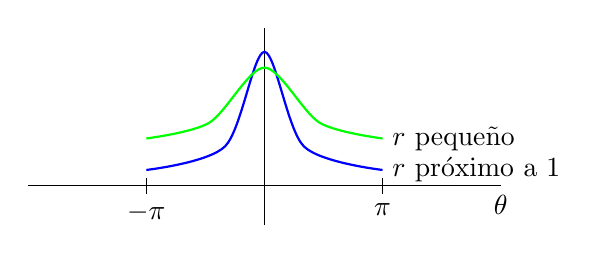
\begin{tikzpicture}

			\draw[-] (-3,0) -- (3,0) node [below] {$\theta$};
			\draw[-] (0,-0.5) -- (0,2);

			\draw[-] (-1.5,0.1) -- (-1.5,-0.1) node[below] {$-\pi$};
			\draw[-] (1.5,0.1) -- (1.5,-0.1) node[below] {$\pi$};

			\draw[blue, thick] plot[smooth] coordinates {(-1.5,0.2) (-0.5,0.5) (0,1.7) (0.5,0.5) (1.5,0.2)};

			\draw[green, thick] plot[smooth] coordinates {(-1.5,0.6) (-0.7,0.8) (0,1.5) (0.7,0.8) (1.5,0.6)};

			\node[right] at (1.5,0.6) {$r$ pequeño};
			\node[right] at (1.5,0.2) {$r$ próximo a 1};

			\end{tikzpicture}
			\end{center}

			Puesto que la función es periódica da lo mismo integrar entre $-\pi$ y $\pi$ que cualquier otro intervalo de tamaño $2\pi$. Todas serán 1.

		\end{itemize}

		\begin{theorem}
			Supongamos que $g$ es una función contínua y $2\pi$-periódica. Entonces:

			\[ \int^\pi_{-\pi} g(s)P(r, \theta-s) ds \convs[][r][1^-] g(\theta) \text{ uniformemente en } [-\pi,\pi] \]

			IMPORTANTE: Este es el primer teorema que vemos en el que se nos indica el límite a parte de darnos convergencia uniforme. Usaremos este teorema como base para ampliar los resultados anteriores.
		\end{theorem}

			\begin{proof}

				\[0 \leq \left| \int_{-\pi}^{\pi} g(s) P(r, \theta-s) - g(\theta))  \right| \]

				Tenemos que $\int\limits_{-\pi}^{\pi} P(r, \theta-s) ds = 1$ por los cálculos anteriores, por lo que la multiplicaremos por lo que ya tenemos:

				\[0 \leq \left| \int_{-\pi}^{\pi} g(s) P(r, \theta-s) - g(\theta))  \int\limits_{-\pi}^{\pi} P(r, \theta-s) ds  \right| \]

				\[ = \left| \int_{-\pi}^\pi (g(s) - g(\theta)) P(r, \theta - s) ds \right|  \leq \int^{\pi}_{-\pi} | g(s) - g(\theta) | P(r, \theta- s) \]

				Hemos podido hacer este paso ya que $P>0$, pero veremos en unos días que no se va a cumplir en otra prueba y tendremos problemas.

				Vamos a descomponer la integral en dos trozos, en uno nos ayudaremos de la continuidad de $g$ y en el otro de la del núcleo.

				\[ = \underbrace{\int_{|\theta-s|< \delta}}_{|g(s) - g(\theta)| \text{ pequeño y }p\text{ grande}} + \underbrace{\int_{|\theta-s| > \delta}}_{|g(s) - g(\theta)| \text{ acotado y }p\text{ pequeño}} \]

				\textbf{i:} Como $g$ es contínua en $[-\pi,\pi]$, intervalo cerrado y acotado. Entonces si $[-\pi,\pi]$ es compacto $\Rightarrow$ $g$ es uniformemente contínua.

				Dado $\epsilon > 0$, $\exists \delta > 0$ tal que si $|\theta-s| < \delta$, entonces $|g(s) - g(\theta)| < \epsilon, \forall \theta$

				\[\Rightarrow \int_{|\theta - s| < \delta} |g(s) - g(\theta) | P(r, \theta - s) ds < \epsilon \int_{|\theta - s| < \delta} P < \epsilon  \underbrace{\int_{-\pi}^{\pi} P}_{= \epsilon}    \]

				Luego tiende a 0, pero hemos fijado $\delta$.

				\textbf{ii:} Par el delta elegido en \textbf{i}, $\int\limits_{|\theta - s | > \delta} |g(s) - g(\theta)| P(r, \theta-s) ds = $

				\[
					\int_{\theta+\delta}^\pi \underbrace{|g(s) - g(\theta)| P(r, \theta-s)}_{(1)} +  \int_{-\pi}^{\theta-\delta} \underbrace{|g(s) - g(\theta)| P(r, \theta-s)}_{(2)}
				\]

				Y tenemos:

				\[ (1) \leq P(r, \theta-(\theta-\delta)) = P(r, -\delta) = P(r, \delta) \leq  \]

				\[\leq P(r, \delta) \int^{\pi}_{\theta+\delta} |g(s) - g(\theta) ds \leq C P(r, \underbrace{\delta}_{> 0}) \convs[][r][1^-] 0  \]

				\[g \text{ continua } \Rightarrow |g| < M \]

				\[ |g(s)  - g(\theta)| \leq |g(s)| + | g(\theta) | \leq 2M \]


				Hemos probado:

				Dado $\epsilon > 0$, $\exists r_0$ tal que si $r \in (r_0,1)$:

				\[ \left| \int_{-\pi}^\pi g(s) P(r, \theta-s) ds - g(\theta)  \right| < \epsilon \quad \forall \theta \]

			\end{proof}

		\textbf{Aplicación}

		\textbf{1:} $f$,$g$ continua, con los mismos coeficientes de Fourier $\Rightarrow f \equiv g$

		\begin{proof}
			\[
				\left. \begin{array}{l}
				f \\
				g
				\end{array} \right\} \rightarrow \alpha_k \rightarrow \sum_k \alpha_k r^{|k|} e^{ik\theta} \left\{ \begin{array}{l}
					\int^{\pi}_{-\pi} f(s) P(r, \theta - s)ds \convs[][r][1^-] f \\
					\int^{\pi}_{-\pi} g(s) P(r, \theta - s)ds \convs[][r][1^-] g
				\end{array} \right.
			\]

			Por unicidad del límite $\Rightarrow f \equiv g$
		\end{proof}

		% clase 2016/02/29

		\textbf{2:} Si tenemos un problema en una circunferencia de radio $a$, hacemos un reescalado:

		% faltan tildas aquí, que no he sabido ponerlas durante la clase
		\[ \gor{W}(\rho, \theta) = W(\frac{\rho}{a},\theta) \quad \rho \in [0,a) \]

		Usando la regla de la cadena llegamos a:

		\[\gor{W}_{\rho \rho} + \frac{1}{\rho} \gor{W}_\rho + \frac{1}{\rho^2} \gor{W}_{\theta \theta} = 0, \quad \rho \in [0,a)  \]

		\[\gor{W}(\rho, \theta) = W(\frac{\rho}{a},\theta) = \int^{\pi}_{-\pi} g(s)\underbrace{P(\frac{\rho}{a},\theta-s)}_{\text{núcleo de Poisson para la bola de radio }a} ds \]

		Como consecuencia del teorema de Poisson tenemos:

		\textbf{i:} \concept{Propiedad\IS de la media}

		 \[u(x,y)|_{(0,0)}  = W(0,\theta) = \int_{-\pi}^\pi g(s) P(0, \theta - s) ds = \frac{1}{2\pi} \int_{-\pi}^\pi g(s) ds \]

		 \[ u_{xx} + u_{yy} = 0\]

		 Las funciones que verifican la condición de laplace (las funciones armónicas) son muy rígidas y verifican que son el promedio de todos los puntos de la circunferencia que les rodea. Son las funciones que aparecen en los equilibrios, por ejemplo, en la función de ondas.

		Lo veremos más adelante, pero se puede imaginar una membrana, que cuando se queda parada, en una posición de equilibrio, los puntos interiores dependen de la forma del bastidor que sujeta la membrana.

		\textbf{ii:} \concept{Propiedad\IS del máximo}:

		Si $m \leq g(\theta) \leq M, \forall \theta \in [-\pi,\pi]$, entonces $m \leq u(x,y) \leq M, \forall (x,y)$

		\[u(x,y) \rightarrow W(r,\theta) = \int_{-\pi}^{\pi} \underbrace{g(s)}_{\in [m,M]} \underbrace{P(r,\theta-s)}_{> 0} ds \begin{cases}
			\leq \int_{-\pi}^{\pi} MP = M \\
			\geq \int_{-\pi}^{\pi} mP = m

		\end{cases} \]

		Una función armónica alcanza mínimo y máximo en el borde, no puede alcanzarlo en el interior.

		\textbf{iii:} $f$,$g$ contínuas, $2\pi$-periódicas si:

		\[ \int_{-\pi}^{\pi} f(s) e^{-iks}ds =
		 \int_{-\pi}^{\pi} f(s) e^{-iks}ds,  \forall k \Rightarrow f \equiv g \]

		\textbf{iv:} \concept{Teorema\IS de aproximación de Weirestrass 1}. Sea f contínua y $2\pi periódica$ entonces existe un polinomio trigonométrico:

		\[T_n (\theta) = \sum_{k = -n}^n c_k e^{ik\theta} \]

		tal que $\forall \epsilon > 0$ existe $n_0$ tal que si $n > n_0$: $|T_n (\theta) - f(\theta)| < \epsilon, \forall \theta \in [-\pi,\pi]$.

		\begin{proof}

			\[f \rightarrow \alpha_k = \int_{-\pi}^\pi f(s) e^{-iks} ds  \]

			\[ \sum_{k=-\infty}^{\infty} \alpha_k r^{|k|} e^{ik\theta} \convs[][r][1^-] f(\theta), \text{ uniformemente.} \]

			Dado $\epsilon > 0$, $\exists \delta > 0$ tal que si $1-\delta < r < 1$ entonces:

			\[ \left| \sum_{k=-\infty}^{\infty} \alpha_k r^{|k|} e^{ik\theta} - f(\theta) \right| < \epsilon, \forall \theta \in [-\pi,\pi]  \]

			Fijamos $r_{*} \in (1-\delta, 1)$

			\textbf{a}

			\[ \left| \sum_{k=-\infty}^{\infty} \alpha_k r^{|k|} e^{ik\theta} - f(\theta) \right| < \epsilon \]

			\[  r_* < 1 \Rightarrow \sum_{k=-\infty}^\infty \alpha_k r_*^{|k|} e^{ik\theta} < \infty \eqreason[\Rightarrow]{Dado $\epsilon > 0, \exists N_0$ tal que si $n \geq n_0$} \sum_{|k| > n} \alpha_k r_*^{|k|} e^{ik\theta} < \epsilon \]

			\textbf{a,b}

			\[ \Rightarrow  \left| \underbrace{\sum_{|k| < k} \alpha_k r_*^{|k|} e^{ik\theta}}_{\text{Suma finita (polinomios trigonométricos)}} - f(\theta) \right| < 2 \epsilon, \forall \theta \in [-\pi,\pi] \]

			Por lo tanto cualquier función contínua se puede aproximar uniformemente por una suma finita de $\alpha_k r^{|k|_* e^{ik\theta}}$.

		\end{proof}

		\textbf{v:} \concept{Teorema\IS de aproximación de Weirestrass 2}

		Dada una función $f$ $2\pi$-preiódica y contínua. $\forall \epsilon > 0 \exists$ un polinomio $p(x)= a_0 + a_1 x + … + a_n x^n $ tal que $|f(x)-P(x)| < \epsilon, \forall x \in [-\pi,\pi]$

		\begin{proof}

			Usar la misma prueba que con el primer teorema de aproximación de Weirestrass

		\end{proof}

		Con esto llegamos a la idea de que si la función $f$ fuera analítica tendríamos que se aproxima uniformemente en un intervalo por su polinomio de Taylor (como los senos y los cosenos)

		Si aproximamos una función con un polinomio trigonométrico, entonces lo tenemos aproximado por muchos términos con senos y cosenos, lo cual son funciones analíticas, que permiten aproximar cada uno de ellos a su polinomio de Taylor del orden que se quiera. Si acotamos cada término con ($\epsilon / $ número de términos) entonces el error total será menor a $\epsilon$.

		Tenemos el problema de que no nos dice como calcular ese $p(x)$, la prueba no es constructiva. Sin embargo, el teorema de funciones analíticas si te da esa solución, pero solo vale para funciones iguales a su polinomio de Taylor.

		\subsection{Identificación del límite con convergencia $L^2$}
		\textbf{Aplicación} al estudio de la convergencia en $L^2$

		$\{\Phi_k\}$ sistema ortonormal en $L^2([-\pi,\pi])$

		Dada $f \in L^2$,

		\[\alpha_k = <f, \Phi_{k}> = \int_{-\pi}^\pi f(s) \overline{\Phi_k(s)} ds  \]

		\[  S_n f = \sum_{|k| < n} (\alpha_k \Phi_k ) \sum_{|k| < n}<f, \Phi_k >\Phi_k \]

		Siendo $\Phi_k(s) = \frac{e^{iks}}{\sqrt{2\pi}}$

		\begin{theorem}

			Entonces sea $T_n$ polinomio trigonométrico de grado $n$:

			\[ \| S_n f - f\|_{L^2} \leq \| T_n - f \|_{L^2} < \epsilon \]

			Y es igual solo si $S_n \equiv T_n$.

		\end{theorem}

			\begin{proof}

				\[ T_n = \sum_{|k| < n} C_k \Phi_k(x) \]

				\[ \| T_n - f \|_{2}^2 = < T_n -f, T_n - f> = < \sum_{|k| < n} C_k \Phi_k(x) - f, \sum_{|k| < n} C_k \Phi_k(x) - f >   \]

				\begin{align*} = < &\sum_{|k| < n} C_k \Phi_k(x), \sum_{|j| < n} C_j \Phi_j(x) > - < \sum_{|k| < n} C_k \Phi_k(x), f> \\ &- <f, \sum_{|j| < n} C_j \Phi_j(x)> + <f,f> \end{align*}

				\[ = \sum_{|k| < n} C_k^2 - \sum_{|k| < n} C_k <\Phi_k(x),f> - \sum_{|j| < n} C_j <\Phi_j(x),f> + \|f\|_2^2  \]


				\[ \| S_n f - f \|_2^2 = … = < \sum_{|k| < n} <f,\Phi_k(x)> \Phi_k -f,  \sum_{|j| < n} <f,\Phi_j(x)> \Phi_j -f>\]

				\[ = … = \|f\|_2^2 - \sum_{|k| < n} |<f,\Phi_k(x)>|^2 \]

				Entonces:

				\[ \| S_n f - f \|_2^2 - \|T_n -f\|_2^2 = … = \sum_{|k| < n} \underbrace{(<f,\Phi_k> - C_k) \overline{(<f,\Phi_k> - C_k)}}_{|<f, \Phi_k> - C_k|^2 < 0}  \]


			\end{proof}

		\textbf{Consecuencias:}

		\begin{itemize}

			\item  \[ f \in L^2 \Rightarrow S_n f \eqexpl[\rightarrow]{$L^2$} f \]

			Lo cual es consecuencia de l resultado anterior junto con el primer teorema de aproximación de Weirestrass

			\item \[ \| S_n f - f \|_{2}^2 - \sum_{|k|<n} | <f, \Phi_k> |^2  \]

			Entonces obtenemos la \concept{Identidad\IS de Parseval}:

			\[ \sum_{k= -\infty}^\infty  |\pesc{f, \Phi_k}|^2 = \|f\|^2_2 \]


		\end{itemize}

		% Revisado hasta aquí

		%clase 2016/03/01


		Aunque hemos hecho trampa, porque hemos aplicado un resultado válido solo para funciones contínuas a funciones que no sabíamos si lo eran. El siguiente teorema nos ayudará con ello:

		\begin{theorem}

			\[ f \in L^2 \Rightarrow S_n f \eqexpl[\rightarrow]{$L^2$} f \]

		\end{theorem}

		\begin{proof}

			\textbf{Caso 1:} Supongamos $f$ contínua.

			Por Weierstrass tenemos que dado $\epsilon > 0$, existe un polinomio $T_n$ tal que $|T_n(s) - f(s)| < \epsilon, \forall s \in [-\pi,\pi]$

			\(
				\int^{\pi}_{-\pi} | S_n f - f |^2 ds \leq \int^\pi_{-\pi} | T_n - f |^2 ds < 2 \pi \epsilon^2 \label{eq:resultadoContinuidadWeierstrass}
			\)

			\textbf{Caso 2:} $f \in L^2 ([-\pi,\pi])$

			Recordemos las dos definiciones equivalentes de $L^2$:
			\begin{itemize}

				\item $L^2 \equiv$ funciones medibles tales que $\int\limits^\pi_{-\pi} |f|^2 dx \leq \infty $

				\item $L^2 \equiv$ cierre del conjunto de las funciones contínuas con la topología inducida por $\|\cdot\|_2$, que se relaciona con \ref{eq:resultadoContinuidadWeierstrass}

			\end{itemize}

			Data $f\in L^2, \exists \set{f_n}$ de funciones contínuas tales que $\|f_n - f\|_2 \convs 0$

			Sea $f_\epsilon$ contínua con $\|f-f_\epsilon\|_2 < \epsilon$:

			Entonces,
			\begin{align*}
			\| S_N f - f \|_2 &= \| S_N f \pm S_N f_\epsilon \pm f_\epsilon - f \|_2 \leq \\
			& \leq \| S_N f - S_N f_\epsilon \|_2 + \| S_N f_\epsilon - f_\epsilon \|_2 + \underbrace{\| f_\epsilon - f \|_2}_{< \epsilon}
			\end{align*}

			Tenemos que $\| S_N f_\epsilon - f_\epsilon \|_2 \convs 0$ por el caso 1; y

			\[ \| S_N f - S_N f_\epsilon \|_2 \eqreason{sumas finitas} \| S_N (f - f_\epsilon) \|_2 \eqreason[\leq]{Bessel} \| f - f_\epsilon \|_2 \]

			Luego tenemos que $\| S_N f - f \|_2 < \epsilon$.

		\end{proof}

		\begin{corol}

		\[ \| S_n f - f \|_2^2 = \|f\|_2^2 - \sum_{-n}^{n} |<f, \Phi_k>|^2\]

		\[\rightarrow \|S_n f - f \|_2 \convs 0 \]

		\[\Rightarrow  \sum_{-\infty}^{\infty} | <f, \Phi>|^2 \eqreason{Parçeval} \|f\|_2^2 \]

		con $\{\Phi_k\}$ ortonormal. Esta fórmula nos permite calcular sumas infinitas.

		\end{corol}


	\subsection{Resultados probados}


		\begin{itemize}

			\item $f \in C^2, 2\pi$-periódica $\Rightarrow S_n f \rightarrow f$ uniformemente

			\item $f\in L^2 \Rightarrow S_n f \eqexpl[\rightarrow]{$L^2$} f$

			\item Bessel, Parseval

			\item Convergencia uniforme de la ``serie modificada'' $\sum\limits_k \alpha_k r^{|k|} e^{ikx}$ (Poisson)

		\end{itemize}


	\subsection{Convergencia puntual}

	\begin{theorem}[Teorema\IS de Dirichlet]

		\[ \{\Phi_k\} = \{\frac{1}{\sqrt{2\pi}} e^{ikx}\}_{k=0, ±1,±2}  \text{ sistema ortonormal en } [-\pi,\pi]\]



	\end{theorem}

	\begin{proof}

		f ``regular''

		\[S_nf = \sum_{k=-n}^{n} <f,\Phi_k> \Phi_k(x) = \sum_{-n}^n \left( \int_{-\pi}^\pi f(s) \frac{1}{\sqrt{2\pi}} e^{-iks} ds \right)  \frac{1}{\sqrt{2\pi}} e^{ikx} \]

		\[ = \sum_{-n}^{n}  \int_{-\pi}^\pi f(s) \frac{1}{2\pi} e^{-ik(s-x)} ds = \int_{-\pi}^{\pi} f(s) \frac{1}{2\pi} \sum_{-n}^n e^{-ik(s-x)} ds \]

		Continuamos con solo el sumatorio de la ecuación anterior: es una progresión geométrica, así que la sabemos calcular (salvo en el límite):

		\[ \frac{1}{2\pi} \sum_{-n}^n e^{-ik(s-x)} = \frac{1}{2\pi} \sum_{-n}^n e^{ik(x-s)} = \frac{1}{2\pi} \sum_{-n}^n \left[\underbrace{e^{i(x-s)} }_{\equiv \rho}\right]^k \]

		\[ \frac{1}{2\pi} \sum_{-n}^n \rho^k = \frac{1}{2\pi} \frac{\rho^{-n} - \rho^{n+1}}{1 -\rho} \]

		\begin{gather*}
		\frac{1}{2\pi}  \sum(e^{it})^k = \frac{1}{2\pi} \frac{e^{-nit}-e^{(n+1)it}}{1-e^{it}} = \frac{1}{2\pi} \frac{e^{-it/2}}{e^{-it/2}} \frac{ e^{-nit}-e^{(n+1)it}}{1-e^{it}} =\\
		= \frac{1}{2\pi} \frac{e^{-(n + 1/2)it}-e^{(n+1/2)it} }{e^{-it/2}-e^{it/2}} \cdot \frac{-1}{-1} = \frac{1}{2\pi} \frac{e^{(n + 1/2)it} - e^{-(n+1/2)it} }{e^{it/2}-e^{-it/2}} = \dots
		\end{gather*}

		\( … = \frac{1}{2\pi} \frac{\sin(n+ \frac{1}{2})t}{\sin(\frac{t}{2})}  \equiv D_n(t) \label{eq:nucleoDirichlet}\)
	\end{proof}

		La expresión \ref{eq:nucleoDirichlet} que hemos obtenido es conocida como \concept{Núcleo\IS de Dirichlet}.

		Pero nos falta por estudiar cuál es la relación entre las propiedades del núcleo de Dirichlet cuando n tiende a infinito y el límite de $S_N f$.




	Comparemos los núcleos de Poisson y Dirichlet:

	\begin{itemize}

		\item Poisson $P(s,t)$ (DIBUJO)

		\item Dirichlet $D_n(t)$ (DIBUJO)

	\end{itemize}

	Como podemos ver, Dirichlet plantea problemas de convergencia.

	El argumento que debemos utilizar debe basarse en las oscilaciones, ya que no tenemos nada más que nos lo permita. Tendremos una integral que queremos hacer tender a cero por culpa de las oscilaciones por culpa de las oscilaciones de dentro, sin tener que meter valor absoluto. El teorema que nos da este tipo de argumentos es el de Riemann-Lebesgue.Veamos:

	Fijando x:

	\( |S_n f(x) - f(x) | = \left| \int_{-\pi}^\pi f(s) D_n (x-s) ds - f(x) \right| \label{eq:dirichletFijandoX} \)

	\textbf{propiedades de $D_n$:}

	\begin{itemize}
		\item $D_n(-t) = D_n(t)$

		\item $\int\limits_{-\pi}^{\pi} D_n(t) = 1, \forall n $

		\[ \int_{-\pi}^\pi  \frac{1}{2\pi} \sum_{-n}^{n} e^{ikt} dt \]

	\end{itemize}


	Entonces:

	\[  \int_{x-\pi}^{x +\pi} f(x-t) D_n(t) dt = \int^{\pi}_{-\pi} f(x-t) D_n(t) dt \]

	\[ \eqref{eq:dirichletFijandoX} = \left| \int_{-\pi}^\pi (f(x-t)-f(x)) \frac{1}{2\pi} \frac{\sin(n+\frac{1}{2})t}{\sin{\frac{t}{2}}} dt \right| \]

	% clase 7/3/2016

	\begin{theorem}[Dirichlet 1]

		Sea $f$ medible y acotada derivable en $x$. Entonces $S_n f(x) \convs f(x)$.

	\end{theorem}

	\begin{proof}

		\[ 0 \leq |S_nf(x) - f(x)  = \left| \int_{-\pi}^{\pi} f(x-t) D_n(t) dt - f(x) \int_{-\pi}^\pi D_n(t) dt \right|  \]

		\[= \left| \int_{-\pi}^\pi (f(x-t)-f(x) D_n(t) dt) \right| = \frac{1}{2\pi} \left| \int_{-\pi}^\pi \frac{f(x-t)-f(x)}{\sin t/2} \frac{\sin(\pi+1/2)t}{\sqrt{\pi}} \right|  \]

		Utilizamos dos teoremas para completar la demostración:

		\begin{itemize}

			\item \textbf{Teorema 1:} $\frac{1}{\sqrt{\pi}} \sin(n + \frac{1}{2}) t $ es una familia ortonormal en $[-\pi,\pi]$

			La demostración se deja como ejercicio al lector

			\item \textbf{Teorema 2:}  En las hipótesis del teorema:

			\[ \frac{f(x-t)-f(x)}{\sin(t/2)} \eqreason[\in]{variable $t$, ($x$ fijo)} L^2 ([-\pi,\pi]) \]

			\begin{proof}
				Sea
				\[ g(t) = \frac{f(x-t)-f(x)}{\sin(t/2)} = \underbrace{\frac{f(x-t)-f(x)}{-t}}_{\convs[ ][t][0] f'(t)} \underbrace{\frac{-t}{\sin(t/2)}}_{\convs[ ][t][0] 2} \]
				Entonces existe un $\delta > 0$ tal que $\| g(t) \| < C$, si $\| t \| < \delta$.

				Observemos que el seno entre $-\pi$ y $\pi$ es impar, y que si quitamos una bola entrada en el 0 de radio $\delta$ tenemos que $\| \frac{1}{\sin(t/2)} \| < k$, si $\| t \| < \delta$.

				Como f es derivable y tenemos un intervalo acotado, tenemos que f está acotada, luego $\| f(x-t) - f(x) \| \leq 2 M$.

				Por tanto, $\| g(t) \| < \gor{C}$, $\forall t \in [-\pi,\pi]$.

				Finalmente,
				\[ \int\limits_{-\pi}^{\pi} \| g(t) \|^2 dt < 2M \gor{C} \implies g \in L^2 \]
			\end{proof}

		\end{itemize}

		Conclusión:

		Lema 1 + Lema 2 + Riemman-Lebesgue $\Rightarrow \left| S_n f(x) - f(x) \right| \rightarrow 0$

	\end{proof}

	\begin{theorem}[Dirichlet 2]

		$f$ medible y acotada. Además solo vamos a permitir discontinuidades de salto, dientes de sierra, etc.. pero vamos a evitar funciones con derivadas infinitas en algún punto. Admitimos límites y derivadas laterales siempre que sean finitos:

		\inputtikz{FuncionesDirichlet}

		\[
		\left.
		\begin{array}{l}
			f(x^+) = \lim_{t \to x^+} f(t) \\
			f(x^-) = \lim_{t \to x^-} f(t) \\
			f'(x^+) = \lim_{h \to 0^+} \frac{f(x+h)-f(x)}{h} \\
			f'(x^-) = \lim_{h \to 0^-} \frac{f(x+h)-f(x)}{h}
		\end{array} \right\} \text{ existen y son finitos.}
		\]

		Entonces: \[ \lim_{n \to \infty} S_nf(x) = \frac{1}{2} \{f(x^+)+f(x^-)\}\]

	\end{theorem}

	\begin{proof}

		\[ 0 \leq | S_n f(x) - \frac{1}{2} \{f(x^+) + f(x^-)\} |\]

		\[ = \left| \int_{-|pi}^\pi f(x-t) D_n (t) dt - \frac{1}{2} f(x^+)- \frac{1}{2} f(x^-) \right|  \]

		\[ \int_{-|pi}^{0} f(x-t) D_n(t)dt + \int_{0}^\pi f(x-t) D_n(t) dt \]

		\[ \left| \underbrace{\int_0^\pi  \{ f(x-t) - f(x^+) \} D_n(t) dt }_{\text{I}} + \underbrace{\int_{-\pi}^{0}  \{ f(x-t) - f(x^-) \} D_n(t) dt }_{\text{II}} \right| \]

		\[\leq | \text{I} | +  |\text{II}| \]

		Si nos fijamos en I:

		\[ I = \frac{1}{2\sqrt{\pi}} \int_{0}^\pi \underbrace{\frac{f(x-t)-f(x)}{\sin(t/2)}}_{=g(t)} \cdot \frac{\sin((n+1/2)t)}{\sqrt{\pi}} \]

		Ojo, $\frac{\sin((n+1/2)t)}{\sqrt{\pi}}$ es un sistema ortonormal en $[-\pi,\pi]$, pero no es siquiera ortogonal en $[0,\pi]$.

		Tenemos
		\[ \int_{0}^\pi \underbrace{g(t)}_{\in L^2} \underbrace{\sin((n+1/2)t)}_{\text{impar}} dt \]
		y lo que debemos hacer es extenderla a $[-\pi,\pi]$.

		Consideramos una función $\gor{g}$, que será la extensión IMPAR de $g$ en el intervalo $[-\pi,\pi]$. Entonces:

		\[ \int_{-\pi}^\pi  \gor{g}(t) \sin(n+1/2)t dt \eqreason[\rightarrow]{Riemann-Lebesgue} 0 \]

		\[ = 2 \int_{0}^\pi g(t) \sin(n \frac{1}{2}) t dt \]


	\end{proof}


	\begin{example}

		Dada $f(x) = x(\pi-x), x \in [0,\pi]$

		(DIBUJO SEMICIRCUNFERENCIA).

		\textbf{1:}

		$f_1 = $ extensión par de $f$:

		(DIBUJO)

		\[\{ 1, \sin{kx}, \cos{kx} \}_{K = ±1,±2,…} \]

		\obs No está normalizada, si quisiéramos usar Parseval, tendríamos que normalizar.

		El teorema de Dirichlet nos garantiza lo siguiente:

		\[
			f_1(x) = \frac{a_0}{2} + \sum_{k=1}^\infty a_k \cos{kx} + \sum_{k=1}^\infty b_k \sin kx
		\]

		Pero tenemos que $b_k = 0 \forall x$:

		\[b_k = \frac{1}{\pi} \int_{-\pi}^{\pi} f_1(x) \sin kx dx = 0 \]

		Tenemos que $a_0$ es:

		\[ a_0 = \frac{1}{\pi} \int_{-\pi}^{\pi} f_1(x) dx = … = \frac{\pi^2}{3} \]

		\[ a_k = \frac{1}{\pi} \int_{-\pi}^{\pi} f_1(x) \cos kx dx\]

		\[ = \frac{2}{\pi} \int_{0}^{\pi} x(\pi - x) \cos kx dx\]

		\[ = \frac{2}{\pi} \left\{ \pi \int_{0}^{\pi} x \cos(kx) dx  - \int_{0^π} x^2 \cos(kx) dx \right\}  \]

		\[ \Rightarrow … \Rightarrow a_k = \begin{cases}
			\frac{-4}{k^2} & k \text{ par} \\
			0 & k \text{ impar}
		\end{cases}  \]

		(FALTA)

		Conclusión:

		\[ x(\pi - x) = \frac{\pi^2}{6} -\sum_n=1^\infty \frac{1}{n^2} \cos(2n) x \]

		En particular, si $x=0$:

		\[ 0 = \frac{π^2}{6}  - \sum_{n=1}^\infty \frac{1}{n^2} \Rightarrow  \sum_{n=1}^\infty \frac{1}{n^2} = \frac{\pi^2}{6} \]

		(FALTA UN DESARROLLO MÁS) %TODO

		\[ \frac{\pi^2}{6} = … = \sum \frac{1}{(2i +1)^2}= 1 + \frac{1}{3^2} + \frac{1}{5^2} + … \]

		\textbf{2:}

		Veamos $f_2$ como la extensión impar de $f$:

		(DIBUJO)

		\[ f_2 \Rightarrow \underbrace{\frac{a_0}{2}}_{0} + \sum_k \underbrace{a_k \cos(kx)}_{0} + \sum_k b_k \sin(kx)  \]

		\[  x(\pi - x) = \sum_{n=1}^{\infty} \frac{8}{n(2n-1)^3} \sin(2_n-1)x  \]

		\[  1 - \frac{1}{3^3} + \frac{1}{5^3} - \frac{1}{7^3} + … = \frac{\pi^3}{32}\]


	\end{example}








% Clase 8/3/2016

Al igual que con el teorema de Dirichlet, podemos ver la aplicación de la identidad de Parçeval, que nos decía que \[ \norm{f}_{L^2}^2 = \sum_{k ∈ ℤ} \abs{\pesc{f, φ_k}}^2 \] con $\set{φ_k}$ nuestro sistema ortonormal.

Consideramos de nuevo la extensión par de $f(x) = x(π-x)$. Podemos calcular y ver que \[ \pesc{\tilde{f}, φ_0} = \frac{1}{\sqrt{2π}} 2 \int_0^π x(π-x) \dif x = \sqrt{\frac{2}{π}} \left(\frac{πx^2}{2} - \frac{x^3}{3}\right|_{x = 0}^π =  \sqrt{\frac{2}{π}} \frac{π^3}{6} \]

Para el resto de los coeficientes, vemos primero que los coeficientes de los senos van a ser $0$ por simetría. En el caso de los cosenos, vemos que \[ \pesc{\tilde{f}, \frac{\cos kx}{\sqrt{π}}} = \frac{2}{\sqrt{π}} \int_{0}^π x(π-x) \cos kx \dif x = \frac{2}{\sqrt{π}} \left(π\int_0^π x \cos kx \dif x - \int_0^π x^2 \cos kx \dif x \right) \]

Resolvemos las dos integrales por separado: \[ \int_0^π x \cos kx \dif x = x \eval{\frac{\sin kx}{k}}_{x=0}^π - \int_0^π \frac{\sin kx}{k} \dif x = \eval{\frac{\cos kx}{k^2}}_{x=0}^π = \frac{(-1)^k - 1}{k^2} \] y la otra integral sale \[ \int_0^π x^2 \cos kx \dif x = \dotsb = \frac{2π}{k^2} (-1)^k \]

Juntando ahora y haciendo más cuentas, queda que \[ \pesc{\tilde{f}, \frac{\cos kx}{\sqrt{π}}} = \frac{2 \sqrt{π}}{k^2}\left(-1 - (-1)^k\right) = \frac{2\sqrt{π}}{k^2} \begin{cases} 0 & k \text{ impar} \\ -2 & k \text{ par} \end{cases} \]

Por otra parte, vemos que \[ \norm{\tilde{f}}^2_{L^2} = \dotsb =\frac{π^5}{15} \]

Así, la identidad de Parçeval nos dice que \[ \frac{π^5}{15} = \left(\sqrt{\frac{2}{π}} \frac{π^3}{6}\right)^2 + \sum_{n=1}^∞ \left(\frac{2\sqrt{π}}{(2n)^2} - ( -2)\right)^2 = \frac{π^5}{18} + \sum_{n=1}^{∞} \frac{π}{n^4} \] y que simplificando \[ \sum_{n=1}^∞ \frac{1}{n^4} = \frac{π^4}{90} \]

Incluso podríamos repetir el resultado que hacíamos antes y sacar todavía más resultados de teoría de números, separando la suma de los pares y los impares \[ \frac{π^4}{90} = \sum_{k ∈ ℕ} \frac{1}{(2k)^4} + \sum_{k ∈ ℕ} \frac{1}{(2k-1)^4} = \sum_{k∈ℕ} \frac{1}{16k^4} + \sum_{k ∈ ℕ} \frac{1}{(2k-1)^4} \] y entonces podemos despejar y ver que \[ \sum_{k ∈ ℕ} \frac{1}{(2k-1)^4} =  \frac{π^4}{90} \frac{15}{16} \]


\subsection{Convergencia puntual para funciones Hölder continuas}

Recuperando lo que teníamos antes, teníamos que la continuidad no nos bastaba para tener convergencia de la serie de Fourier. Du Bois-Raymond construía un ejemplo de una función continua cuya serie no convergía en un punto, y Kolmogorov iba un poco más allá con una función continua cuya serie divergía en todo punto.

Pediremos algo más que continuidad:

\begin{defn}[Función\IS continua Hölder] Se dice que una función $\appl{f}{X}{ℝ}$ es Hölder continua si existe un $α ∈ [0,1]$ y $K ∈ ℝ$ tal que $∀t,s ∈ X$ (por ejemplo, $X = [-π, π]$) se cumple que \[ \abs{f(t) -f(s)} < K \abs{t-s}^α\]
\end{defn}

\begin{theorem} Sea $\appl{f}{X}{ℝ}$ una función Hölder continua. Entonces su serie de Fourier converge en todo punto a $f(x)$.
\end{theorem}

El punto de partida es el de siempre: tenemos que \[ \sum_{n = 0}^∞ a_n ≝ \lim_{N \to ∞} S_N\qquad\quad S_N = \sum_{n=0}^N a_n\]

Para tratar esta suma introducimos el concepto de la \concept{Sumabilidad\IS Cèsaro}, definiendo las series de la media de las sumas parciales \[ σ_N = \frac{S_0 + \dotsb +  S_N}{N+1}\]

Estas series tienen límite si lo tienen las sumas parciales:

\begin{theorem} Si $\lim S_N = L$, entonces $\lim σ_N = L$. El recíproco no siempre es cierto.
\end{theorem}

Un ejemplo es ver que la serie $(-1)^n$ sí es sumable según Cèsaro, aunque no en el sentido habitual. Lo peculiar de esta serie es que oscila, y esto nos hace pensar que también se podría aplicar a las series de Fourier, que igualmente oscilan con los senos y cosenos.

\begin{theorem} \[ σ_Nf = \int_{-π}^π f(x) F_N(x-t) \dif t \], donde $F_N$ son los núcleos de Féjer, que no son más que el promedio de los núcleos de Dirichlet \[ F_N(t) = \frac{1}{N+1} \sum_{k=0}^{N-1} D_k(t) = \frac{1}{N+1} \left(\frac{\sin\left(\frac{N+1}{2}\right) t}{\sin \frac{t}{2}}\right)^2\]
\end{theorem}

Lo interesante del núcleo de Féjer es que es positivo y que nos permitirá hacer cuentas igual que hacíamos con el núcleo de Poisson.

\subsubsection{Aplicación a las EDPs}

\textbf{Aplicación a la ecuación del calor}

Recordamos la ecuación que teníamos del calor: \begin{align*}
u_t - u_{xx} = 0 & \quad x ∈ (0,L),\, t > 0 \\
u(0,t) = u(L,t) = 0 & \quad  t > 0 \\
u(x,0) = f(x)
\end{align*}

Usando el método de separación de variables, llegábamos a que la solución era \[ u(x,t) \qeq \sum_{k ∈ ℤ} a_k e^{-\left(\frac{kπ}{L}\right)^2 t} \sin \frac{kπ}{L} x \], donde \[ f(x) \qeq \sum_{k ∈ ℤ} a_k \sin \frac{kπ}{L} x \]

Teníamos tres interpretaciones: convergencia uniforme si tenemos $f ∈ C^2$ periódica, convergencia en sentido $L^2$ y convergencia puntual con el teorema de Dirichlet.

Un teorema (que habría que poner un poquito mejor):

\begin{theorem} Si $\sum f_k = f$ con convergencia uniforme y $\sum f_k' = g$, entonces $f$ es derivable y $f' = g$.
\end{theorem}

Con esto, podemos derivar la solución $u(x,t)$ y vemos que \[ u_t = \sum_{k ∈ ℤ} a_k \left[-\left(\frac{kπ}{L}\right)^2\right]  e^{-\left(\frac{kπ}{L}\right)^2 t} \sin \frac{kπ}{L} x \]

Aplicamos aquí el siguiente lema:

\begin{lemma} Sean $α, β > 0$. Entonces si la siguiente suma converge: \[ \sum_{k ∈ ℤ} k^α e^{-k^2β} < ∞\], entonces converge uniformemente.
\end{lemma}

Tenemos que efectivamente $u_t$ es esa serie con convergencia uniforme. Si hacemos la derivada con $u_{xx}$ nos quedará algo con convergencia uniformemente igualmente.





% Clase 9/3/2016


		\textbf{Aplicación a la ecuación de ondas}

			\[  \begin{cases}
				u_{tt} - u_{xx} = 0 \\
				u(0,t) = u(L,t) = 0 \\
				u(x,0) = f(x) \\
				u_t(x,0) = g(x) \equiv 0
				\end{cases}
			\]

			Por separación de variables y como $g \equiv 0$:

			\[
			\begin{cases}
				u(x,t) = \sum_{k=1}^\infty a_k \cos(\frac{k\pi}{L}t) \sin(\frac{k\pi}{L}x) \\
				\text{ donde } f(x) = \sum_{k=1}^\infty a_k \sin(\frac{k\pi}{L}x)
			\end{cases}
			\]

			Realizamos la extensión impar de $f$ al intervalo $[-L,L] \rightarrow$ los coeficientes de los cosenos se anulan.

			Entonces podemos escribir la serie de $u$. Como veíamos, tenemos 3 interpretaciones del $=$ dependiendo del tipo de convergencia que estemos hablando.

			Toda la regularidad y convergencia que vamos a conseguir viene de los $a_k$, ya que no tenemos exponenciales, solo senos y cosenos que oscilan. Lo que quiere decir que la serie que vamos a obtener será ``buena'' si la serie dato es buena y mala si no.

			El criterio que teníamos para regularidad era el decaimiento de la serie, como los senos y cosenos están acotados y su valor absoluto será como máximo uno, entonces sus factores (los $a_k$) son los que influyen en esa convergencia. Esto se puede extrapolar a la fórmula D'Alambert (\ref{eq:DALEMBERT}).


			Miremos una extensión de la serie de los $a_k$:

			\[a_1 \cos\left(\frac{\pi}{L}t \right) \sin\left(\frac{\pi}{L}x \right) + a_2 \cos\left(\frac{2\pi}{L}t \right) \sin\left(\frac{2\pi}{L}x \right) + a_3 \cos\left(\frac{3\pi}{L}t \right) \sin\left(\frac{3\pi}{L}x \right) + …\]


			(3 DIBUJOS)


			Por Riemann-Lebesgue tenemos que $a_k \to 0$.

	\subsection{Extensiones}

		\subsubsection{Transformada de Fourier}
			Estudiamos el espectro de la función. Lo usamos cuando no conocemos la longitud de la cuerda.
					$f(x)$, L desconocido.
					\[\int_{-\infty}^\infty f(x) e^{-i} \xi^x dx = \gor{f} (\xi) \]

		\subsubsection{Transformada de Fourier discreta} (DFT)

			Supongamos que tenemos $f(x)$, $2\pi$-periódica.

			\[ f(x) = \sum_{k=-\infty}^\infty c_k e^{ikx}\]

			Realizamos una grabación digital de sonido realizando un muestreo. Es decir, el micrófono nos da el valor de la función para muchos tiempos discretos.

			(DIBUJO SAMPLING)

			Nuestro propósito es resumir esa información para poder guardarla de forma comprimida. Intentaremos hacer una interpolación para reconstruir la función inicial $f$. Después calcularemos la serie de Fourier de esta, y por último truncaremos las frecuencias no audibles para comprimir.

			Este proceso sería muy costoso así que en vez de hacer todos los pasos uno por uno vamos a intentar no tener que pasar por el mundo contínuo.

			Tenemos unos datos;

			En el intervalo $[0,2\pi]$ dividido en $N$ trozos:

			\[x_j = \frac{2\pi}{N}j, \quad j=0,1,2,…,N-1\]

			Y el sampling que hemos realizado:

			\[ y_j = f(\frac{2\pi}{N}j)\]


			\textbf{Idea 1}

			Supongamos que existe:

			\[f(x) = \sum_{k=-\infty}^\infty c_k e^{ikx} \]

			\[ y_0 = f(x_0) = f(0) = \sum_{k=-\infty}^\infty c_k \]
			\[ y_1 = f(x_1) = f\left(\frac{2\pi}{N}\right) = \sum_{k=-\infty}^\infty c_k \left( e^{i\frac{2\pi}{N}} \right)^k \eqreason{$e^{i\frac{2\pi}{N}} \equiv \omega $} \sum_{k=-\infty}^\infty c_k \omega^k \]
			\[ y_p = f(x_p) = f\left(\frac{2\pi}{N}p\right) = \sum_{k=-\infty}^\infty c_k \left(\omega^p\right)^k \]



			Tenemos $N ecuaciones$ e infinitas incógnitas $C_k$. Los $C_k$ son valores exactos pero podemos reducir el problema a encontrar valores aproximados $z_k$. Veamos el sistema aproximado:

			\[y_0 = \sum_{k=0}^N-1 z_k\]
			\[y_1 = \sum_{k=0}^N-1 z_k \omega^k\]
			\[y_{N-1} = \sum_{k=0}^N-1 z_k \left(\omega^{N-1}\right)^k\]


			\obs
			\[ \omega = e^{i \frac{2\pi}{N}}  \]

			(FALTA COMPLETAR)


			Todo lo que tenemos es periódico así que cualquier bloque de longitud $N$ nos vale (es equivalente). Porque todos os coeficientes son $N$-periódicos. Suponiendo que los datos $\{y_i\}$ también los extiendo de manera $N$-periódica a izquierda y derecha. Tenemos que cualquier bloque de longitud $N$ es equivalente.

			\[k=0,1,2,…,N-1\]
			\[k = -\frac{N}{2}, -\frac{N}{2}+1, … , \frac{N}{2}\]


			Formulación matricial:

			\[ \bar{Y} = \left(
			\begin{matrix}
				1 & 1 & 1 & … & 1 \\
				1 & \omega & \omega^2 & … & \omega^{N-1} \\
				· & \omega^2 & \omega^4 & … & \omega^{(N-1)2} \\
				· & · & · & · & · \\
				1 & \omega^{N-1} & (\omega^2)^{N-1} & … & \omega^{(N-1)(N-1)}
			\end{matrix} \right) \bar{Z}
			\]

			Ortogonalidad:

			\[ \sum_{s=0}^{N-1} \omega^{js} \omega^{-LS} = \begin{cases}
			0 & L \neq j\\
			N & L = j
			\end{cases} \]

			(FALTA UNA COSILLA Y UN POCO DE EXPLICACIÓN)

			Veamos la demostración

			\begin{proof}

			\[ \omega^{js} \omega^{-LS} = \omega^{(j-L)S} = e^{i\frac{2\pi}{N}(j-L)s}  \]

			(FALTA TERMINAR)

			\end{proof}

			% clase 14/3/2016

			% La clase empieza con un comentario que amplia información de una sección anterior, que no he copiado.

			\textbf{Aplicación:} cálculo de $\bar{z}$.

				\[ y_j\omega^{-js} = \sum_{k=0}^{n-1} z_k \omega^{jk} \omega^{-js} \]

				\[ \sum_{j=0}^{n-1} y_j \omega^{-js} = \sum_{j=0}^{n-1} \sum_{k=0}^{n-1} z_k \omega^{jk} \omega^{-js} = \]\[ = \sum_{k=0} z_k \sum_{j=0}^{n-1} \omega^{jk} \omega^{-js} = \begin{cases}
					0 & s \neq k\\
					N & s = k  \end{cases} \]

				\textbf{Conclusión}

				\[ \sum_{j=0}^{n-1} y_j \omega^{-js} = n z_s   \]
				\[ z_s = \frac{1}{n} \sum_{j=0}^{n-1} y_j \omega^{-js}   \]
				\[ y_j = \sum_{k=0}^{n-1} z_k \omega^{jk} \]
				\[ \{\bar{z}\} \equiv \text{Transformada discreta de orden n de } \{\bar{y}\} \]

				\[ \bar{z} = F_n (\bar{y}) \]



			\textbf{Idea 2:}

			\[f(x) = \sum_{k=-\infty}^{\infty} c_k e^{ikx} \]
			\[c_k= \frac{1}{2\pi} \int_0^{2\pi} f(x) e^{-ikx} dx ≈ \frac{1}{2\pi} \sum_{j=0}^{n-1} f(x_j) e^{-ikxj} \frac{2\pi}{n}  \]
			\[ = \frac{1}{N} \sum_{j=0}^{n-1}  y_j \omega^{-kj} \equiv z_k  \]

			Tomando $k = n$:

			\[c_n \underbrace{\eqexpl[≈]{?}}_{\text{En general no}} \frac{1}{n} \sum_{j=0}^{n-1} y_j \omega^{-Nj}  \eqreason{$\omega^n \equiv 1$} \frac{1}{n} \sum_{j=0}^{n-1} y_j \omega^{0j} = z_0   \]

			En general $z_{n+l} = z_{l}$.

			Esta es una aproximación válida si  $k << n$.

			(DIBUJO ALIASING)


			\textbf{Relación precisa entre $\{c_k\}$ y $\{z_k\}$}

			\[ f(x) = \sum_{L=-\infty}^\infty c_L e^{iLx}  \]

			\[ z_k = \frac{1}{N}  \sum_{j=0}^{n-1} y_j \omega^{-kj} = \frac{1}{n} \sum_{j=0}^{n-1}  f(x_j) \omega^{-kj} = \frac{1}{n} \sum_{j=0}^{n-1} f\left( \frac{2\pi}{n} j \right) \omega^{-kj}  \]

			\[  = \frac{1}{n} \sum_{j=0}^{n-1} \sum_{L=-\infty}^{\infty} c_L e^{iL\frac{2\pi}{n}j} \omega^{-kj} = \frac{1}{n} \sum_{l=-\infty}^{\infty} c_l \sum_{j=0}^{n-1} \omega^{lj} \omega^{-kj} \]


			No podemos aplicar tal cual el teorema de ortogonalidad porque la $l$ no va entre 0 y $n$. Pero podemos descomponer la suma en trozos de longitud $n$. En cada uno de ellos solo uno de los sumandos será distinto de 0.

			(DIBUJO RECTA DIVIDIDA)


			\[ \omega^{Lj} = \omega^{(L+n)j} = \omega^{(L+2n)j} … \]

			\[ \frac{1}{n} \sum_{L=-\infty}^{\infty} c_L \sum_{j=0}^{n-1} \omega^{Lj} \omega^{-kj} = \frac{1}{n} n \{ c_k + c_{k+n} + c_{k+2n} + … \}  \]

			\[ z_k = c_k + c_{k+n} + c_{k+2n} + c_{k+3n} + … = \sum_{k \mod n} c_k  \]

			Por Riemman-Lebesgue: $C_k \convs[][k] 0$

			Esto nos indica que el muestreo puede hacer que una onda de mucha frecuencia en nuestros datos baje de frecuencia al tomar la transformada de Fourier.


			\obs Veamos una función $f(x) = \sum\limits_{k=-\infty}^{\infty} c_k e^{ikx}$.

			\[ \left|  f - \sum_{k=-\infty}^{\infty} c_k e^{ikx} \right| = 0 \]
			\[ = \left|  f - \sum_{|k|\leq n} + \sum_{|k| > n} \right| \geq \left|  f- \sum_{|k| \leq n} \right| - \left| \sum_{|k| > n} \right| \]

			\[ \left| f- \sum_{|k| \leq n} c_k e^{ikx} \right| \leq \left| \sum_{|k| > n} c_k e^{ikx} \right| \leq \sum_{|k| > n} |c_k|  \]

			Este es el error exacto que cometemos en el desarrollo de Fourier, en base a las $c$s. Tenemos este teorema que nos dice que si hacemos ese mismo cálculo con las $z$s, el error no es muy malo:

			\begin{theorem}
				\[ \left| f - \sum_{|k|< n} z_k e^{ikx}  \right| \leq 2 \sum_{|k| > n |c_k| } \]
			\end{theorem}


			\subsubsubsection{Cálculo efectivo (FFT)}

			\[ \bar{u} = (u_0, u_1, … u_{n-1}) \rightarrow F_n (\bar{u})  \]
			\[ \bar{v} = (v_0, v_1, … v_{n-1}) \rightarrow F_n (\bar{v})  \]

			Entonces:

			\[ \bar{y} = (y_0,y_1,…,y_{2n-1}) \equiv (u_0,v_0,u_1,v_1, … u_{n-1},v_{n-1})  \]

			Pero que pasa con $f_{2n}(\bar{y})$?

			Tenemos

			\[ \left(F_{2n} (\bar{y})\right)_k = \left(F_{n} (\bar{u})\right)_k + \left(F_{n} (\bar{v})\right)_k \omega_{2n}^{-k}, k=0,1,…,n-1 \]

			\[ \left(F_{2n} (\bar{y})\right)_{k+n} = \left(F_{n} (\bar{u})\right)_k - \left(F_{n} (\bar{v})\right)_k \omega_{2n}^{-k}, k=0,1,…,n-1 \]

			\[ (\omega_{2n} = e^{i\frac{2\pi}{2n}}, \omega_{n} = e^{i \frac{2\pi}{n}})  \]

			\begin{proof}

				\[ w_{2n}^2 = \omega_{n} \]

				Separamos la suma en indices pares e impares y listo.

			\end{proof}

			\textbf{Método FFT}

			(DIBUJO ÁRBOL FFT)

			Este método es $O(n \log n)$.









